\documentclass[10pt, titlepage]{article}
% preámbulo
\usepackage{lmodern}
\usepackage[T1]{fontenc}
\usepackage[document]{ragged2e}
\usepackage[spanish,activeacute]{babel}
\usepackage{mathtools}
\usepackage{hyperref}
\usepackage{xcolor}
\usepackage{geometry}
\usepackage{float}

\geometry{
    a4paper,
    left=25mm,
    right=25mm,
    top=25mm,
    bottom=25mm
}
\usepackage{fancyhdr}

\pagestyle{fancy}
\fancyhf{}
\rhead{Eduardo Arroyo Ramírez \\ i12arrae@uco.es}
\lhead{Introducción al Aprendizaje Automático \\ Memoria de prácticas}
\lfoot{\rightmark}
\rfoot{Página \thepage}

\def\code#1{\texttt{#1}}

\hypersetup{
    colorlinks=true,
    linkcolor=blue,
    filecolor=magenta,
    urlcolor=cyan,
}

\title{Introducción al Aprendizaje Automático - Memoria de prácticas}
\author{Eduardo Arroyo Ramírez}

\begin{document}

\graphicspath{ {Practica1/capturas/} }

\makeatletter
\begin{titlepage}
    \begin{center}
        {\scshape\Large Escuela Politécnica Superior \par}
        \vspace{0.5cm}
        {\scshape\large Universidad de Córdoba \par}
        \vspace{4cm}
        {\scshape\Huge Introducción al Aprendizaje Automático \par}
        \vspace{0.5cm}
        {\itshape\Large Memoria de prácticas \par}
    \end{center}
    \vspace{13cm}
    \begin{flushright}
        \@author\space \\
        i12arrae@uco.es \\
        Curso 2019/2020
    \end{flushright}
\end{titlepage}

\tableofcontents
\listoffigures
\listoftables

% Aquí comienza el cuerpo del documento
\justify
%\setlength{\parindent}{1.5cm}
\part{Práctica 1}
\section{Actividad 1-1}\label{p11}
\begin{center}
    \parbox{12cm}{\justify\textit{
        Elija 3 bases de datos de la UCI Machine Learning Repository de las que hay en Moodle y transformelas a .arff, indicando en cada una de ellas qué procedimiento ha seguido.
    }}
\end{center}

\subsection{Consideraciones generales}\label{ssc:consideraciones-generales}
Para la realización de la tarea he tomado la decisión de editar manualmente los archivos utilizando Visual Studio Code y guardarlos con la extensión \code{.arff}. El paso a csv utilizando excel que se ha sugerido en clase supone varios cambios de formato en los que pueden aparecer diversos problemas como conflictos entre el separador de columnas CSV y el separador de decimales o miles, problemas con el carácter de salto de línea, codificación, etc.

Para conocer los identificadores y tipos de los atributos de cada base de datos he consultado el archivo \code{.names} del directorio de descarga de cada base de datos, que contiene el listado de campos con su nombre, su tipo y sus posibles valores, si procede. He consultado la especificación del formato \code{.arff} en la \href{https://www.cs.waikato.ac.nz/ml/weka/arff.html}{página correspondiente del manual de weka}. Como puede comprobarse en la figura \ref{fig:ejemplo-arff}, un archivo \code{.arff} consta de tres secciones:
\begin{figure}[ht]
    \centering
    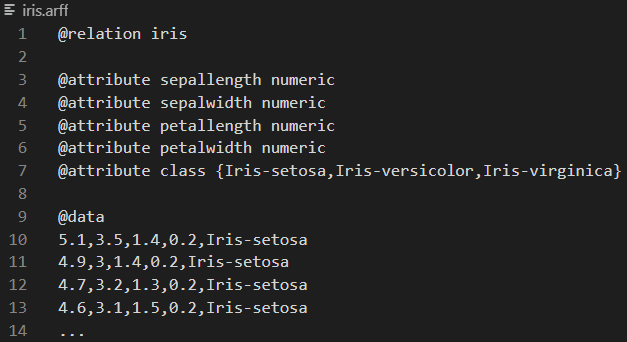
\includegraphics[scale=0.5]{ejemplo-archivo-arff}
    \caption{Ejemplo de archivo \code{.arff}}
    \label{fig:ejemplo-arff}
\end{figure}
\begin{enumerate}
    \item Identificación de la base de datos. Se trata de una línea con el token \code{@relation} seguido por un espacio y el nombre de la base de datos. Por ejemplo: \code{@relation breast-cancer}.
    \item Identificación de los atributos. Tantas líneas como atributos tenga la base de datos, cada una comienza con el token \code{@atribute} seguido del nombre del atributo y el tipo. Los tipos pueden ser:
        \begin{itemize}
            \item Numéricos: \code{@attribute <nombre\string_atributo>\space numeric}
            \item Cadenas de texto: \code{@attribute <nombre\string_atributo> \space string}
            \item Listas de etiquetas: \code{@attribute <nombre\string_atributo> \space\string{valor\string_1, valor\string_2, \dots\string}}
            \item Fechas: \code{@attribute <nombre\string_atributo>\space date [formato\string_de\string_fecha]}. El formato de fecha es opcional, y por defecto acepta ISO-8601 y ``yyyy-MM-dd'T'HH:mm:ss''.
        \end{itemize}
    \item Bloque de datos. Esta sección se inicia con una línea que contiene únicamente palabra clave \code{@data}. A continuación se encontrarán los registros dispuestos en líneas y con sus atributos separados por comas, en el mismo orden en que se han especificado en la cabecera:
    \begin{center}
        \parbox{5.1cm}{\code{@data \\
            v1a1, v1a2, \dots, v1aN \\
            v2a1, v2a2, \dots, v2aN \\
            \dots \\
            vMa1, vMa2, \dots, vMaN
        }}
    \end{center}

\end{enumerate}

\subsection{Base de datos \code{breast-cancer}}
Tras aplicar el tratamiento mencionado en el apartado \ref{ssc:consideraciones-generales} al archivo \code{breast-cancer.data} se ha obtenido el fichero \code{.arff} (fig. \ref{fig:breast-cancer-arff}) y una vez cargado en Weka (fig. \ref{fig:breast-cancer-weka}) y se han obtenido las siguientes conclusiones:

\begin{enumerate}
    \item La base de datos tiene 10 atributos, de los cuales el primero es la clase, que toma los valores ``no-recurrence-events'' y ``recurrence-events''. Convendría colocar la clase al final, que es su lugar por defecto.
    \item Los atributos son nominales basados en etiquetas (por ejemplo breast\_quad, menopause\dots) o en rangos numéricos (inv\_nodes, tumor\_size\dots). El atributo deg\_malig se podría poner como numérico ya que parece representar el grado de malignidad en un rango de 1 a 3, por lo que hay una distancia distinta entre los elementos (por ejemplo 1-2 y 1-3).
\end{enumerate}

\begin{figure}[H]
    \centering
    \begin{minipage}{0.49\textwidth}
        \centering
        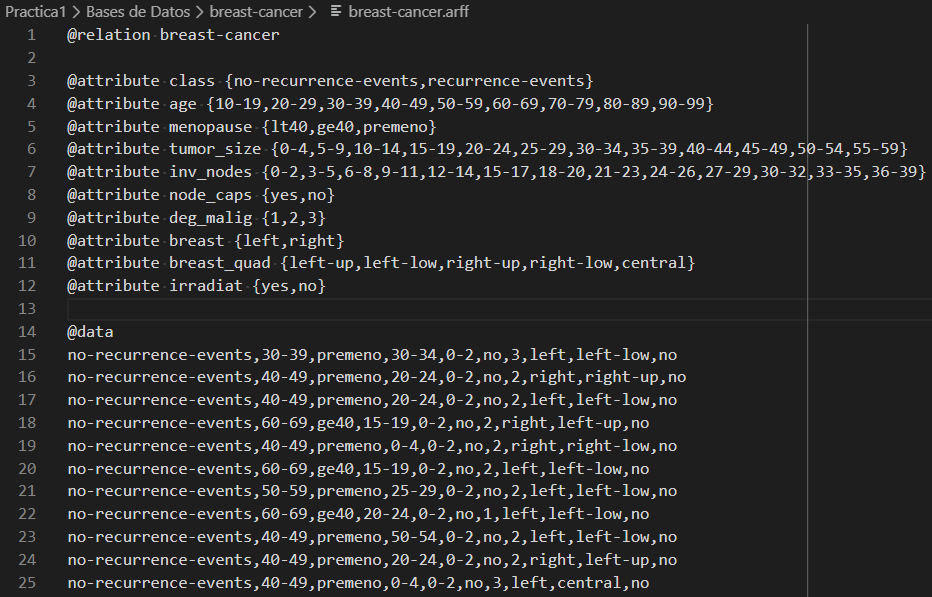
\includegraphics[scale=0.3]{breast-cancer-arff}
        \caption{Captura de \code{breast-cancer.arff}.}
        \label{fig:breast-cancer-arff}
    \end{minipage}
    \begin{minipage}{0.49\textwidth}
        \centering
        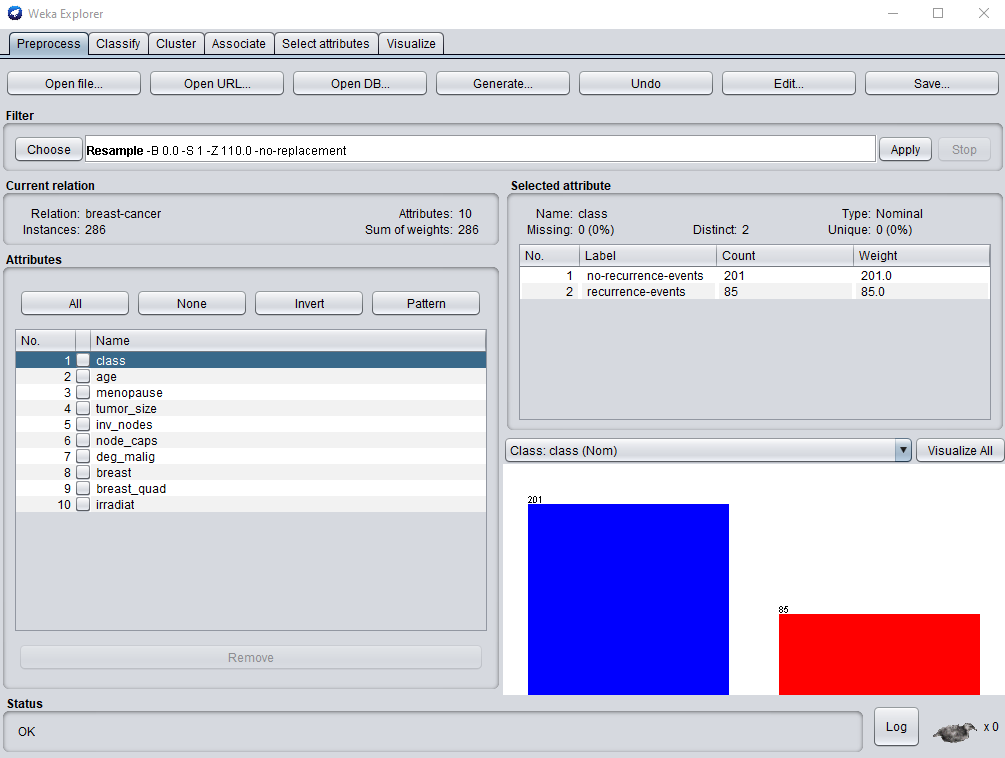
\includegraphics[scale=0.29]{breast-cancer-weka}
        \caption{Archivo \code{breast-cancer.arff} cargado en Weka.}
        \label{fig:breast-cancer-weka}
    \end{minipage}
\end{figure}

\subsection{Base de datos \code{dermatology}}
Tras aplicar el tratamiento mencionado en el apartado \ref{ssc:consideraciones-generales} al archivo \code{dermatology.data} se ha obtenido el fichero \code{.arff} (fig. \ref{fig:dermatology-arff}) y una vez cargado en Weka (fig. \ref{fig:dermatology-weka}) y se han obtenido las siguientes conclusiones:

\begin{enumerate}
    \item La base de datos tiene 34 atributos independientes y una clase. En total hay 366 patrones.
    \item La mayoría los atributos son de tipo numérico con valores [0-3]. En la descripción se indica que los valores indican un grado obtenido de un análisis. El caso del atributo family-history es una excepción, ya que es nominal con valores 0 y 1 y representa si alguna de las enfermedades ha sido observada en la familia. Otra excepción es la edad, que siendo numérica, no está restringida al rango anterior.
    \item La clase toma valores de 1 a 6 y cada valor representa un diagnóstico diferente, por lo que es un dato nominal.
\end{enumerate}
\begin{figure}[H]
    \centering
    \begin{minipage}{0.45\textwidth}
        \centering
        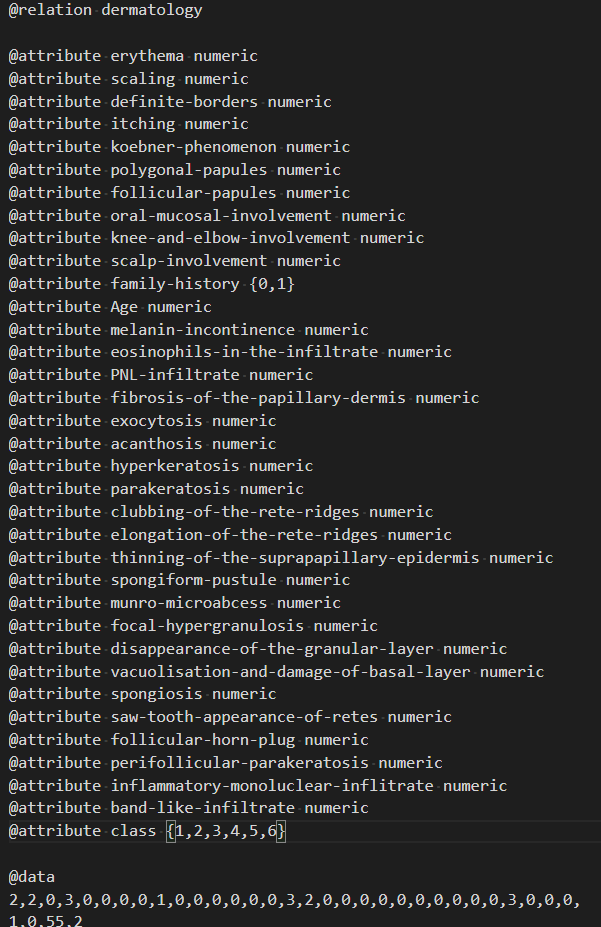
\includegraphics[scale=0.40]{dermatology-arff}
        \caption{Captura de \code{dermatology.arff}.}
        \label{fig:dermatology-arff}
    \end{minipage}\hfill
    \begin{minipage}{0.55\textwidth}
        \centering
        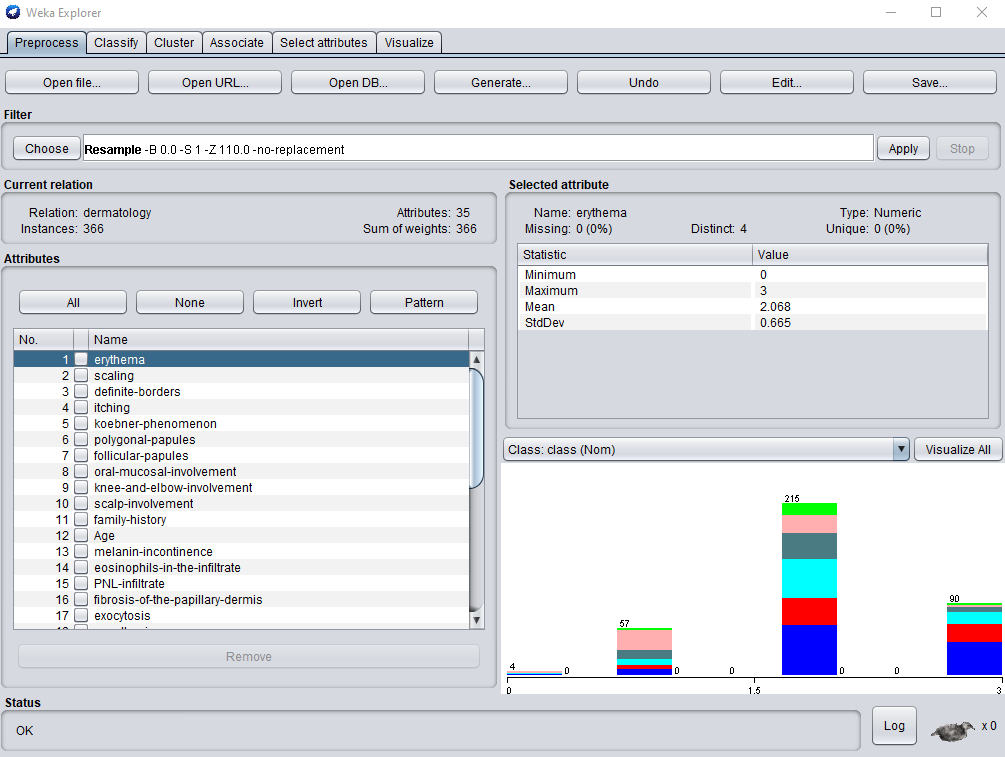
\includegraphics[scale=0.33]{dermatology-weka}
        \caption{Archivo \code{dermatology.arff} cargado en Weka.}
        \label{fig:dermatology-weka}
    \end{minipage}
\end{figure}


\subsection{Base de datos \code{wine}}
Tras aplicar el tratamiento mencionado en el apartado \ref{ssc:consideraciones-generales} al archivo \code{wine.data} se ha obtenido el fichero \code{.arff} (fig. \ref{fig:wine-arff}) y una vez cargado en Weka (fig. \ref{fig:wine-weka}) y se han obtenido las siguientes conclusiones:

\begin{enumerate}
\item La base de datos tiene 13 atributos independientes y una clase al principio.
\item Los atributos son numéricos continuos.
\item La clase toma valores 1, 2 o 3 con frecuencias 59, 71 y 48 respectivamente. Es un dato nominal
\end{enumerate}


\begin{figure}[H]
    \centering
    \begin{minipage}{0.49\textwidth}
        \centering
        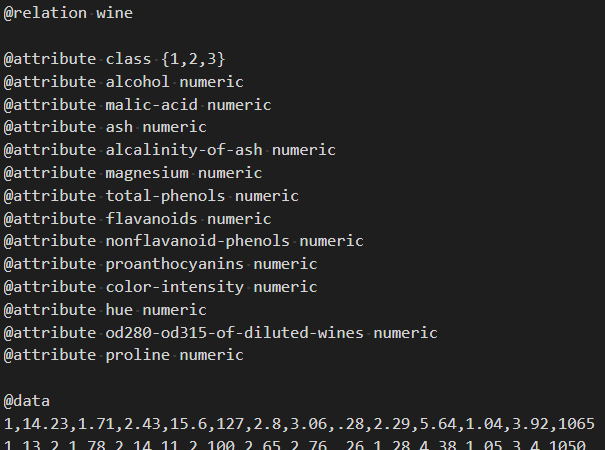
\includegraphics[scale=0.45]{wine-arff}
        \caption{Captura del archivo \code{wine.arff}.}
        \label{fig:wine-arff}
    \end{minipage}
    \begin{minipage}{0.49\textwidth}
        \centering
        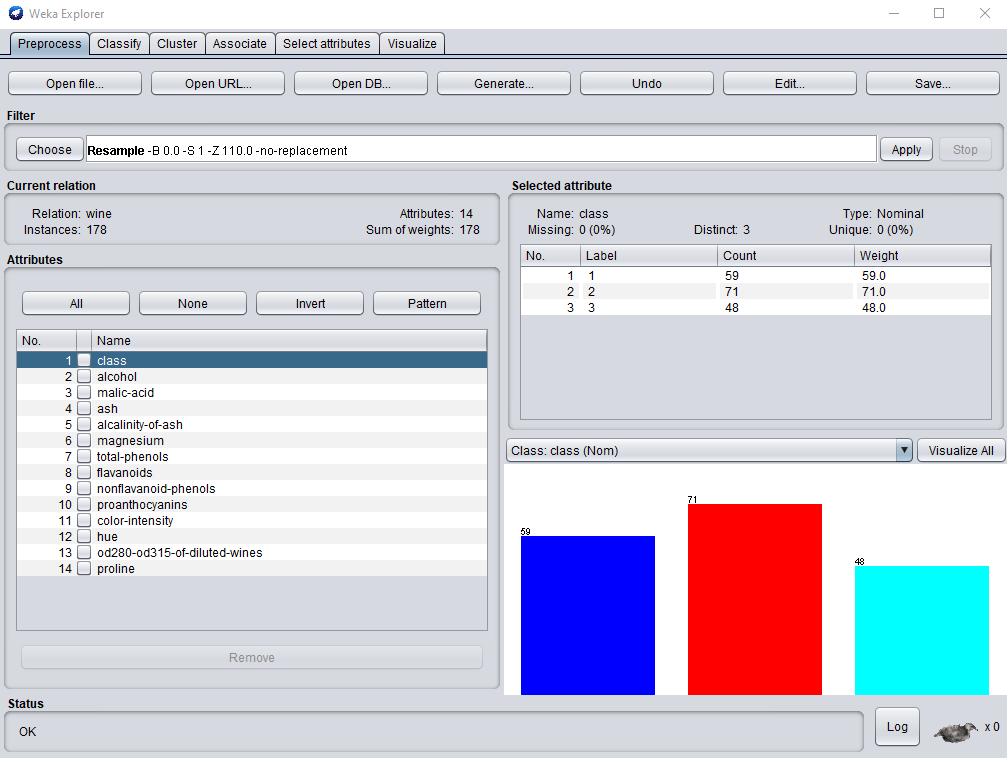
\includegraphics[scale=0.29]{wine-weka}
        \caption{Archivo \code{wine.arff} cargado en Weka.}
        \label{fig:wine-weka}
    \end{minipage}
\end{figure}


%-------------------------------------------------------------------------------
%-------------------------------------------------------------------------------
%-------------------------------------------------------------------------------
\clearpage
\section{Actividad 1-2}\label{p12}
\begin{center}
    \parbox{12cm}{\justify\textit{Elija 3 filtros No Supervisados de los que aparecen listados, expliquelos y describa cómo quedan los datos antes y después al aplicarlos sobre una o varias bases de datos.
    \begin{itemize}
        \item Consulte el UCI Machine Learning Repository para una descripción de la base de datos y la transformación a \code{.arff}
        \item Si no puede aplicar un filtro elegido en ninguna base de datos describa por qué, y constrúyase una base de datos ficticia y pequeña donde si pueda aplicarlo.
        \item Use capturas de pantalla, salidas de Weka y todo lo que considere necesario para sus ejercicios.
        \item La puntuación variará en función de la argumentación y dificultad de los filtros elegidos.
        \begin{enumerate}
            \item filters/unsupervised/attribute/Normalize
            \item filters/unsupervised/attribute/ReplaceMissingValues
            \item filters/unsupervised/attributes/NominalToBinary
            \item filters/unsupervised/intance/RemoveDuplicates
            \item filters/unsupervised/instance/Resample
            \item filters/unsupervised/attribute/Remove
            \item filters/unsupervised/attributes/RemoveUseless
        \end{enumerate}
    \end{itemize}
    }}
\end{center}

\subsection{filters/unsupervised/instance/Resample}
\label{ssc:unsupervised-resample}
Según la información que proporciona Weka, este filtro produce un conjunto de datos mediante un remuestreo de la base de datos original. Este remuestreo no supervisado se utiliza para aumentar el número de patrones (\textbf{oversampling}) mediante la creación de duplicados de patrones existentes o para reducirlo (\textbf{undersampling}) mediante la eliminación de patrones aleatorios. La selección de patrones para oversampling se puede hacer con o sin repetición. Si es sin repetición, un patrón duplicado no podrá ser seleccionado de nuevo para su duplicación.

Para ilustrar el comportamiento del filtro observaremos cómo cambian las frecuencias relativas en las clases tras realizar diversos undersamplings y oversamplings. La hipótesis es que las frecuencias relativas no se mantendrán constantes ya que el filtro elimina o duplica patrones al azar. En Weka, se ha cargado la base de datos \code{dermatology.arff}. En la base de datos hay inicialmente 366 patrones repartidos en 6 clases con las frecuencias que se pueden ver en la columna ``Frec. Orig.'' del cuadro \ref{tab:unsupervised-resample-undersample-dist}. Posteriormente, se ha seleccionado el filtro Resample no supervisado: \code{unsupervised/instance/Resample}.

El filtro Resample no supervisado cuenta con los siguientes parámetros de configuración (ver fig. \ref{fig:unsupervised-resample}):

\begin{itemize}
    \item \code{invertSelection False/True}: Invierte la selección (descartados por seleccionados).
    \item \code{noReplacement True/False}: Deshabilita el reemplazo de instancias, esto es, al seleccionar instancias para duplicar, permite o no que la misma instancia sea seleccionada más de una vez. Esto sólo tiene sentido al hacer oversampling (sampleSizePercent>100).
    \item \code{randomSeed (núm 1)}: Semilla para la selección aleatoria.
    \item \code{sampleSizePercent (núm 100)}: Tamaño del conjunto resultante como \% del original.
\end{itemize}

\begin{figure}[ht]
    \centering
    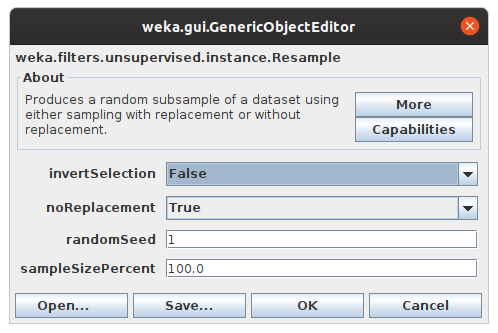
\includegraphics[scale=0.35]{unsupervised-resample}
    \caption{Configuración del filtro \code{unsupervised/Resmaple}.}
    \label{fig:unsupervised-resample}
\end{figure}

Para este ejercicio se han establecido los siguientes valores de configuración:
\begin {itemize}
    \item \code{randomSeed=50}
    \item \code{noReplacement=True}
    \item \code{invertSelection=False}
    \item \code{sampleSizePercent=\{75, 50, 25\}}.
\end{itemize}

En el cuadro \ref{tab:unsupervised-resample-undersample-dist} y figura \ref{fig:unsupervised-resample-undersample-dist} se muestra la distribución de las clases al utilizar el filtro para realizar \textbf{undersampling} reduciendo el conjunto al 75\%, al 50\% y al 25\%. Cada resample se ha realizado sobre el conjunto original. El proceso ha sido: aplicar el filtro, tomar los datos, deshacer, siguiente.
\begin{table}[ht]
    \centering
    \begin{tabular}{|r|rr|rr|rr|rr|}
        \hline
        \multicolumn{1}{|l|}{Clase} & \multicolumn{2}{r|}{Frec. Orig.} & \multicolumn{2}{r|}{Frec. US75} & \multicolumn{2}{r|}{Frec. US50} & \multicolumn{2}{r|}{Frec. US25} \\ 
        \hline
        1 & 112 & 30,60\% & 87 & 31,75\% & 62 & 33,88\% & 31 & 34,07\% \\
        2 & 61  & 16,67\% & 43 & 15,69\% & 25 & 13,66\% & 13 & 14,29\% \\
        3 & 72  & 19,67\% & 54 & 19,71\% & 37 & 20,22\% & 16 & 17,58\% \\
        4 & 49  & 13,39\% & 37 & 13,50\% & 24 & 13,11\% & 12 & 13,19\% \\
        5 & 52  & 14,21\% & 39 & 14,23\% & 27 & 14,75\% & 16 & 17,58\% \\
        6 & 20  & 5,46\%  & 14 & 5,11\%  & 8  & 4,37\%  & 3  & 3,30\%  \\
        \hline 
        Total\footnote{Porcentajes respecto al tamaño número inicial de patrones} & 366 & 100\% & 274 & 74,86\% & 183 & 50,00\% & 91 & 24,86\% \\
        \hline
    \end{tabular}
    \caption{Frecuencias de clases con diferentes undersamplings}
    \label{tab:unsupervised-resample-undersample-dist}
\end{table}
\begin{figure}[H]
    \centering
    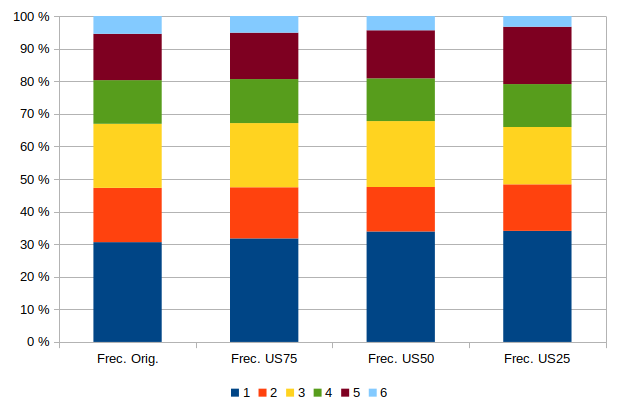
\includegraphics[scale=0.45]{unsupervised-resample-undersample-dist}
    \caption{Frecuencias de clases con diferentes undersamplings}
    \label{fig:unsupervised-resample-undersample-dist}
\end{figure}

Siguiendo la misma dinámica que con el undersampling, se ha realizado un oversampling del conjunto original utilizando el filtro Resample no supervisado, observado que sólo tiene efecto cuando el parámetro \code{noReplacement} se pone a valor \code{False}. En el cuadro \ref{tab:unsupervised-resample-oversample-dist} y figura \ref{fig:unsupervised-resample-oversample-dist} se pueden ver las frecuencias de las diferentes clases al realizar oversamplings al 125\%, 150\%, 175\% y 200\%.

\begin{table}[ht]
    \centering
    \begin{tabular}{|r|rr|rr|rr|rr|rr|}
        \hline
        \multicolumn{1}{|c|}{Clase} & \multicolumn{2}{c|}{Frec. Orig.} & \multicolumn{2}{c|}{Frec. OS125} & \multicolumn{2}{c|}{Frec. OS150} & \multicolumn{2}{c|}{Frec. OS175} & \multicolumn{2}{c|}{Frec. OS200} \\ 
        \hline
        1 & 112 & 30,60\% & 136 & 29,76\% & 168 & 30,60\% & 190 & 29,69\% & 216 & 29,51\% \\
        2 & 61  & 16,67\% & 66  & 14,44\% & 83  & 15,12\% & 100 & 15,63\% & 114 & 15,57\% \\
        3 & 72  & 19,67\% & 89  & 19,47\% & 107 & 19,49\% & 127 & 19,84\% & 149 & 20,36\% \\
        4 & 49  & 13,39\% & 58  & 12,69\% & 68  & 12,39\% & 80  & 12,50\% & 88  & 12,02\% \\
        5 & 52  & 14,21\% & 79  & 17,29\% & 91  & 16,58\% & 104 & 16,25\% & 118 & 16,12\% \\
        6 & 20  & 5,46\%  & 29  & 6,35\%  & 32  & 5,83\%  & 39  & 6,09\%  & 47  & 6,42\%  \\
        \hline
        Total\footnote{Porcentajes respecto al tamaño muestral inicial} & 366 & 100,00 \% & 457 & 124,86 \% & 549          & 150,00 \% & 640 & 174,86 \% & 732 & 200,00 \% \\
        \hline
    \end{tabular}
    \caption{Frecuencias de clases con diferentes oversamplings}
    \label{tab:unsupervised-resample-oversample-dist}
\end{table}
\begin{figure}[ht]
    \centering
    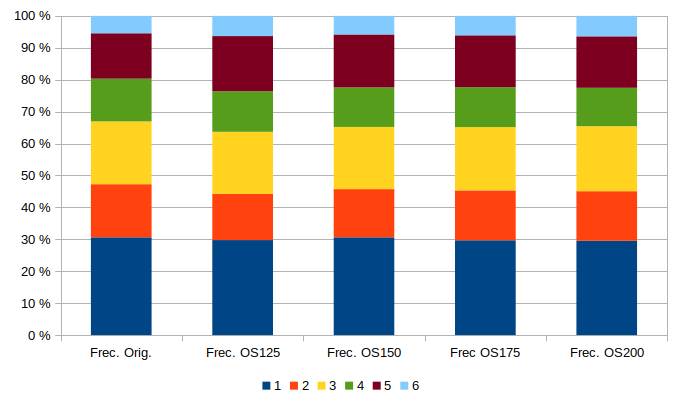
\includegraphics[scale=0.45]{unsupervised-resample-oversample-dist}
    \caption{Frecuencias de clases con diferentes oversamplings}
    \label{fig:unsupervised-resample-oversample-dist}
\end{figure}

Al comparar la frecuencia de cada clase tras las distintas aplicaciones del filtro (fig. \ref{fig:unsupervised-resample-undersample-dist} y \ref{fig:unsupervised-resample-oversample-dist}), se puede observar que varían para los distintos valores de \code{sampleSizePercent}, aunque no demasiado. Dado que se trata de un filtro no supervisado (no tiene en cuenta la clase a la hora de eliminar o crear patrones), este hecho puede deberse a que la base de datos es bastante homogénea en el sentido de que los patrones de cada clase se encuentran distribuidos regularmente a lo largo de la base de datos. En casos de undersampling extremo (ej.: reducción al 4\%) se observa cómo llegan a desaparecer todos los patrones de algunas clases.

En el apartado \ref{ssc:supervised-resample} se probará el filtro supervisado equivalente para comparar las frecuencias obtenidas. Sería lógico suponer que en el filtro supervisado, las frecuencias relativas de las clases variarán menos que en el supervisado según se va reduciendo la muestra.

\subsection{filters/unsupervised/attributes/NominalToBinary}
El filtro no supervisado NominalToBinary reemplaza cada atributo nominal que tenga más de dos valores distintos, por tantos atributos binarios como valores diferentes tenga el atributo original. Estos atributos binarios tendrán valor 1 si el patrón tenía el valor correspondiente al atributo binario en el atributo original y 0 si no. Este proceso se denomina binarización.

\begin{figure}[ht]
    \centering
    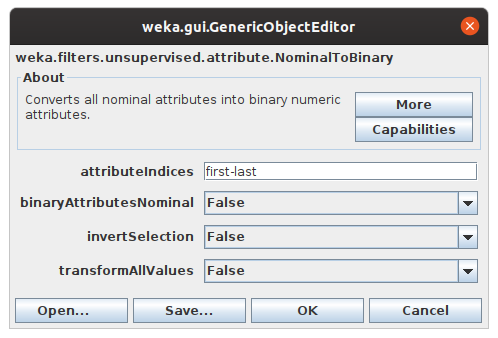
\includegraphics[scale=0.36]{unsupervised-nominal-to-binary}
    \caption{Configuración del filtro \code{unsupervised/NominalToBinary}.}
    \label{fig:unsupervised-nominal-to-binary}
\end{figure}

El filtro NominalToBinary, cuyo formulario de configuración puede verse en la figura \ref{fig:unsupervised-nominal-to-binary} cuenta con los siguientes parámetros:

\begin{itemize}
    \item \code{attributeIndices ([first-last])}: indica el rango de atributos que se van a binarizar. Se especifican los índices o rangos de índices separados por comas. También son válidos los valores ``first'' y ``last''.
    \item \code{binaryAttributesNominal False/True}: Permite establecer si los valores de los nuevos atributos binarios serán valores de tipo 0-1 o si o nominal f-t.
    \item \code{invertSelection False/True}: Si es False, se binarizan los atributos indicados en attributeIndices. Si es True, se binarizan sólo los que no están especificados en dicho parámetro.
    \item \code{transformAllValues False/True}: Si es True, se procesan también los atributos nominales con sólo dos valores.
\end{itemize}

Para ilustrar el funcionamiento de este filtro se ha cargado la base de datos \code{breast-cancer.arff} en Weka y se ha aplicado el filtro a los campos 3 y 6. El primero es nominal con tres valores y el segundo es nominal con dos valores (fig. \ref{fig:breast-cancer-attribute-menopause} y \ref{fig:breast-cancer-attribute-node-caps}). La configuración del filtro es \code{attributeIndices=3,6}, \code{binaryAttributesNominal=True}, \code{invertSelection=False} y \code{transformAllValues=False}, por lo tanto se espera que reemplace el atributo \code{menopause} por tres atributos, uno por cada uno de los tres valores que toma, y que el atributo \code{code\_caps} se quede intacto ya que salvo que se ponga \code{transformAllValues=True} o \code{binaryAttributesNominal=False}, este filtro no altera los atributos nominales de dos valores.

\begin{figure}[ht]
    \centering
    \begin{minipage}{0.50\textwidth}
        \centering
        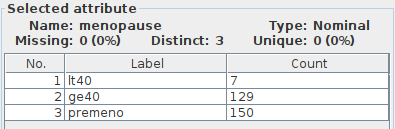
\includegraphics[scale=0.55]{breast-cancer-attribute-menopause}
        \caption{Información del atributo \code{menopause}}
        \label{fig:breast-cancer-attribute-menopause}
    \end{minipage}\hfill
    \begin{minipage}{0.50\textwidth}
        \centering
        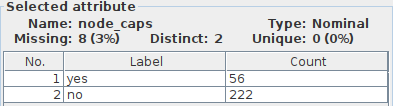
\includegraphics[scale=0.52]{breast-cancer-attribute-node-caps}
        \caption{Información del atributo \code{node\_caps}}
        \label{fig:breast-cancer-attribute-node-caps}
    \end{minipage}
\end{figure}

Los resultados obtenidos (fig. \ref{fig:breast-cancer-nominal-to-binary-1}) confirman la hipótesis:
\begin{itemize}
    \item El filtro ha reemplazado el atributo \code{menopause} por tres campos binarios, uno por cada valor diferente que tomaba el atributo original: \code{menopause=lt40}, \code{menopause=ge40} y \code{menopause=premeno}.
    \item El filtro no ha alterado el atributo \code{node\_caps} porque sólo toma dos valores diferentes.
    \item Las distribuciones de los nuevos campos son coherentes con la distribución del campo original, es decir: hay 7 patrones con valor 1 en \code{menopause=lt40}, hay 129 patrones con valor 1 en \code{menopause=ge40} y hay 150 patrones con valor 1 en \code{menopause=premeno}.
\end{itemize}

\begin{figure}[ht]
    \centering
    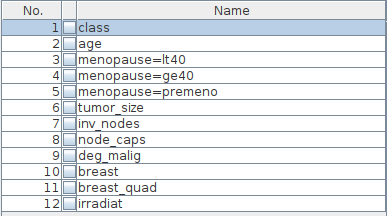
\includegraphics[scale=0.5]{breast-cancer-nominal-to-binary-1}
    \caption{Campos tras aplicar \code{NominalToBinary}.}
    \label{fig:breast-cancer-nominal-to-binary-1}
\end{figure}

Se ha observado que si se establece a False el parámetro \code{}, altera los atributos nominales con dos valores, reemplazando los valores nominales por 0 y 1 pero sin reemplazar el atributo. Para que reemplace el atributo como hace con los nominales de más de dos valores, debe ponerse a True el parámetro \code{transformAllValues}.

\subsection{filters/unsupervised/attributes/RemoveUseless}
El filtro no supervisado RemoveUseless elimina los atributos de la base de datos que no varían o que lo hacen demasiado. Es decir, elimina todos los atributos con valor constante o cuya variación excede el porcentaje indicado en el parámetro \code{maximumVariancePercentageAllowed}. Para calcular la variación de un atributo se aplica la siguiente fórmula:
\begin{equation*}
\text{Variación}=\dfrac{\text{Nº Valores Distintos}}{\text{Nº Valores Total}}\cdot100
\end{equation*}

El formulario de configuración de este filtro puede verse en la figura \ref{fig:unsupervised-remove-useless}.

\begin{figure}[ht]
    \centering
    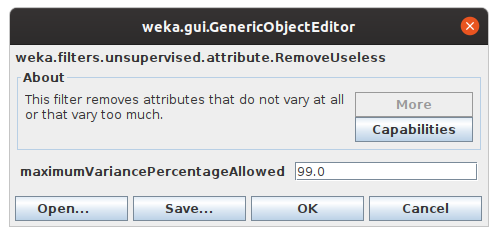
\includegraphics[scale=0.5]{unsupervised-remove-useless}
    \caption{Configuración del filtro \code{unsupervised/RemoveUseless}}
    \label{fig:unsupervised-remove-useless}
\end{figure}

Para probar este filtro se va a componer una base de datos de ejemplo con 200 patrones y 6 atributos más una clase. Los atributos tienen las siguientes características:
\begin{enumerate}
    \item \code{atr1} nominal binario con valores SI/NO. Todos los patrones tienen valor NO. Los datos que arroja Weka sobre este atributo se ven en la fig. \ref{fig:unsupervised-remove-useless-atr1}.
    \item \code{atr2} nominal binario con valores SI/NO. Todos los patrones tienen valor NO excepto uno con valor SI. Este atributo se ha puesto como control del primero, para comprobar que no es eliminado por el filtro. Los datos que arroja Weka sobre este atributo se ven en la fig. \ref{fig:unsupervised-remove-useless-atr2}.    
    \item \code{atr3} numérico. Todos los patrones tienen valor 7.0. Es el mismo caso que \code{atr1} para numérico. Se espera que el filtro elimine este campo también. Los datos que arroja Weka sobre este atributo se ven en la fig. \ref{fig:unsupervised-remove-useless-atr3}.
    \item \code{atr4} nominal con valores \code{a1\dots a200}. Cada atributo toma un valor diferente. La tasa de variación es $\frac{200}{200}\cdot100=100$. Los datos que arroja Weka sobre este atributo se ven en la fig. \ref{fig:unsupervised-remove-useless-atr3}.
    \item \code{atr5} nominal con valores \code{b1\dots b199}. Cada atributo toma un valor diferente salvo los dos últimos que son iguales. La tasa de variación es $\frac{199}{200}\cdot100=99,5$. Los datos que arroja Weka sobre este atributo se ven en la fig. \ref{fig:unsupervised-remove-useless-atr5}.
    \item \code{atr6} nominal con valores \code{a1\dots a200}. Cada atributo toma un valor diferente salvo los tres últimos que son iguales. La tasa de variación es $\frac{198}{200}\cdot100=99$. Los datos que arroja Weka sobre este atributo se ven en la fig. \ref{fig:unsupervised-remove-useless-atr6}.
\end{enumerate}

\begin{figure}[H]
    \centering
    \begin{minipage}{0.50\textwidth}
        \centering
        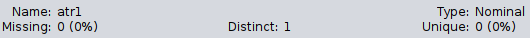
\includegraphics[scale=0.4]{unsupervised-remove-useless-attr1}
        \caption{Atributo \code{atr1}}
        \label{fig:unsupervised-remove-useless-atr1}
    \end{minipage}\hfill
    \begin{minipage}{0.50\textwidth}
        \centering
        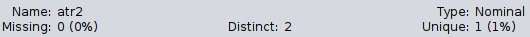
\includegraphics[scale=0.4]{unsupervised-remove-useless-attr2}
        \caption{Atributo \code{atr2}}
        \label{fig:unsupervised-remove-useless-atr2}
    \end{minipage}
\end{figure}
\begin{figure}[H]
    \centering
    \begin{minipage}{0.50\textwidth}
        \centering
        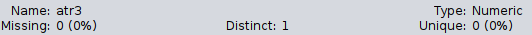
\includegraphics[scale=0.4]{unsupervised-remove-useless-attr3}
        \caption{Atributo \code{atr3}}
        \label{fig:unsupervised-remove-useless-atr3}
    \end{minipage}\hfill
    \begin{minipage}{0.50\textwidth}
        \centering
        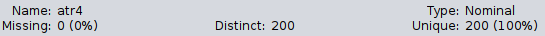
\includegraphics[scale=0.4]{unsupervised-remove-useless-attr4}
        \caption{Atributo \code{atr4}}
        \label{fig:unsupervised-remove-useless-atr4}
    \end{minipage}
\end{figure}
\begin{figure}[H]
    \centering
    \begin{minipage}{0.50\textwidth}
        \centering
        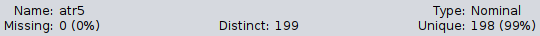
\includegraphics[scale=0.4]{unsupervised-remove-useless-attr5}
        \caption{Atributo \code{atr5}}
        \label{fig:unsupervised-remove-useless-atr5}
    \end{minipage}\hfill
    \begin{minipage}{0.50\textwidth}
        \centering
        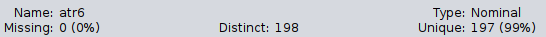
\includegraphics[scale=0.4]{unsupervised-remove-useless-attr6}
        \caption{Atributo \code{atr6}}
        \label{fig:unsupervised-remove-useless-atr6}
    \end{minipage}
\end{figure}

Se aplicará la configuración por defecto del filtro, que especifica el valor 99 para el parámetro \code{maximumVaiancePercentajeAllowed}. Se espera que el filtro elimine los atributos 1 y 3 por ser constantes y 4 y 5 por tener una tasa de variación superior al 99\% configurado en el parámetro. Como se puede comprobar en la figura \ref{fig:unsupervised-remove-useless-aplicado}, el filtro se ha comportado como se esperaba: eliminando los atributos \code{atr1}, \code{atr3}, \code{atr4} y \code{atr5} y manteniendo \code{atr2} y \code{atr6}.

\begin{figure}[H]
    \centering
    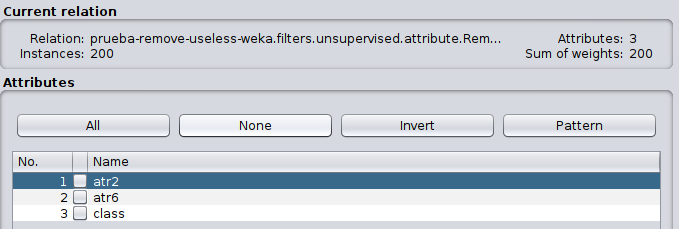
\includegraphics[scale=0.5]{unsupervised-remove-useless-aplicado}
    \caption{Resultado de aplicar el filtro \code{RemoveUseless}.}
    \label{fig:unsupervised-remove-useless-aplicado}
\end{figure}

%-------------------------------------------------------------------------------
%-------------------------------------------------------------------------------
%-------------------------------------------------------------------------------
\clearpage
\section{Actividad 1-3}\label{p13}
\begin{center}
    \parbox{12cm}{\justify\textit{Elija 3 filtros Supervisados de los que aparecen listados, expliquelos y describa cómo quedan los datos antes y después al aplicarlos sobre una o varias bases de datos.
    \begin{itemize}
        \item Consulte el UCI Machine Learning Repository para una descripción de la base de datos y la transformación a \code{.arff}
        \item Si no puede aplicar un filtro elegido en ninguna base de datos describa por qué, y constrúyase una base de datos ficticia y pequeña donde si pueda aplicarlo.
        \item Use capturas de pantalla, salidas de Weka y todo lo que considere necesario para sus ejercicios.
        \item La puntuación variará en función de la argumentación y dificultad de los filtros elegidos.
        \begin{enumerate}
            \item filters/supervised/attribute/Discretize
            \item filters/supervised/attribute/NominalToBinary
            \item filters/supervised/instance/SpreadSubsample
            \item filters/supervised/instance/ClassBalancer
            \item filters/supervised/instance/Resample
        \end{enumerate}
    \end{itemize}
    }}
\end{center}


\subsection{filters/supervised/instance/Resample}
\label{ssc:supervised-resample}
El filtro Resample supervisado produce un conjunto de datos mediante un remuestreo de la base de datos original teniendo en cuenta la clase. Este remuestreo supervisado se utiliza para aumentar el número de patrones (\textbf{oversampling}) mediante la creación de duplicados de patrones existentes o para reducirlo (\textbf{undersampling}) mediante la eliminación de patrones manteniendo ciertas proporciones entre los patrones de cada clase. La selección de patrones para oversampling se puede hacer con o sin repetición. Si es sin repetición, un patrón duplicado no podrá ser seleccionado de nuevo para su duplicación. Según la documentación, la clase debe ser de tipo nominal para poder utilizar este filtro. De lo contrario, deberemos utilizar la versión no supervisada \ref{ssc:unsupervised-resample}.

Para comprobar el comportamiento del filtro observaremos cómo cambian las frecuencias relativas en las clases tras realizar diversos undersamplings y oversamplings en función del valor del parámetro \code{biasToUniformClass}. La hipótesis es que para el valor 0 la distribución de la clase se mantendrá igual mientras que para valor 1 se igualarán. Para valores intermedios del parámetro, mientras más cerca de 1, producirán un resultado más uniforme. En Weka, se ha cargado la base de datos \code{dermatology.arff}. En la base de datos hay inicialmente 366 patrones repartidos en 6 clases con las frecuencias que se pueden ver en la columna ``Frec. Orig.'' del cuadro \ref{tab:unsupervised-resample-oversample-dist}. Posteriormente, se ha seleccionado el filtro Resample supervisado: \code{supervised/instance/Resample} cuyo formulario de configuración se puede ver en la figura \ref{fig:supervised-resample}.

\begin{figure}[ht]
    \centering
    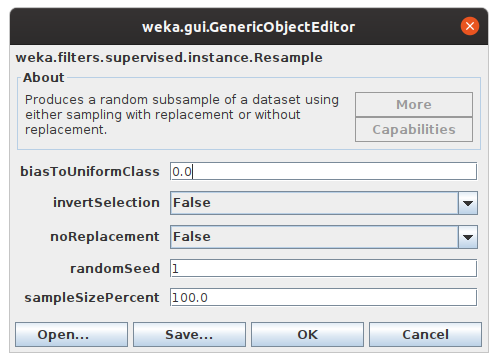
\includegraphics[scale=0.5]{supervised-resample}
    \caption{Configuración del filtro \code{supervised/Resmaple}.}
    \label{fig:supervised-resample}
\end{figure}
El filtro Resample supervisado cuenta con los siguientes parámetros:

\begin{itemize}
    \item \code{biasToUniformClass (núm [0.0-1.0])}: Establece el tipo de sesgo del remuestreo: para 0 se mantiene distribución original de la clase, para 1, la distribución es uniforme.
    \item \code{invertSelection False/True}: Invierte la selección (descartados por seleccionados).
    \item \code{noReplacement True/False}: Deshabilita el reemplazo de instancias, esto es, al seleccionar instancias para duplicar, permite o no que la misma instancia sea seleccionada más de una vez. Esto sólo tiene sentido al hacer oversampling (\code{sampleSizePercent>100}).
    \item \code{randomSeed (núm 1)}: Semilla para la selección aleatoria.
    \item \code{sampleSizePercent (núm 100)}: Tamaño del conjunto resultante como \% del original.
\end{itemize}

Para este ejercicio se han establecido los siguientes valores de configuración:
\begin {itemize}
    \item \code{biasToUniformClass=\{0.0, 1.0\}}
    \item \code{randomSeed=50}
    \item \code{noReplacement=True}
    \item \code{invertSelection=False}
    \item \code{sampleSizePercent=\{33, 66, 150, 200\}}.
\end{itemize}

En el cuadro \ref{tab:supervised-resample-bias0-dist} aparecen los datos de los distintos resamples realizados y se comparan las frecuencias de las clases con las originales. Estos datos se han obtenido con \code{biasToUniformClass=0} y como se puede observar en el gráfico \ref{fig:supervised-resample-bias0-dist}, las proporciones son bastante similares a las originales.

\begin{table}[ht]
    \centering
    \begin{tabular}{|r|rr|rr|
    >{\columncolor[HTML]{C0C0C0}}r 
    >{\columncolor[HTML]{C0C0C0}}r |rr|rr|}
    \hline
    \multicolumn{1}{|c|}{Clase} &
      \multicolumn{2}{c|}{Frec. US33} &
      \multicolumn{2}{c|}{Frec. US66} &
      \multicolumn{2}{c|}{\cellcolor[HTML]{C0C0C0}Frec. Orig.} &
      \multicolumn{2}{c|}{Frec. OS150} &
      \multicolumn{2}{c|}{Frec. OS200} \\ \hline
      1     & 30  & 25,00\% & 59  & 24,48\% & 112 & 30,60\%  & 142 & 25,87\%  & 196 & 26,78\% \\
      2     & 20  & 16,67\% & 34  & 14,11\% & 61  & 16,67\%  & 92  & 16,76\%  & 122 & 16,67\% \\
      3     & 29  & 24,17\% & 63  & 26,14\% & 72  & 19,67\%  & 120 & 21,86\%  & 153 & 20,90\% \\
      4     & 15  & 12,50\% & 31  & 12,86\% & 49  & 13,39\%  & 78  & 14,21\%  & 97  & 13,25\% \\
      5     & 23  & 19,17\% & 40  & 16,60\% & 52  & 14,21\%  & 87  & 15,85\%  & 122 & 16,67\% \\
      6     & 3   & 2,50\%  & 14  & 5,81\%  & 20  & 5,46\%   & 30  & 5,46\%   & 42  & 5,74\%  \\ \hline
      Total\footnote{Porcentajes respecto al tamaño muestral inicial} & 120 & 32,79\% & 241 & 65,85\% & 366 & 100,00\% & 549 & 150,00\% & 732 & 200,00\% \\ \hline
    \end{tabular}
    \caption{Frecuencias de clases con diferentes resamples y \code{biasToUniformClass=0}}
    \label{tab:supervised-resample-bias0-dist}
\end{table}
\begin{figure}[H]
    \centering
    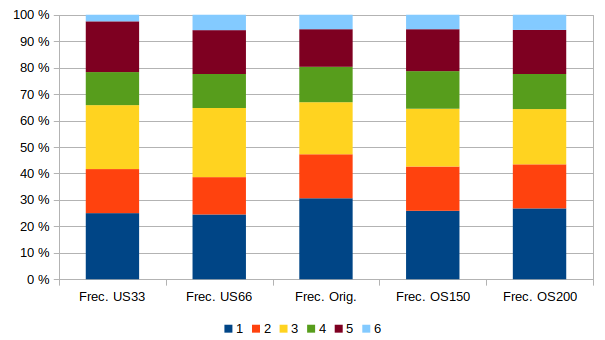
\includegraphics[scale=0.63]{supervised-resample-bias0-dist}
    \caption{Frecuencias de clases al hacer resample con \code{biasToUniformClass=0}}
    \label{fig:supervised-resample-bias0-dist}
\end{figure}

En la tabla \ref{tab:supervised-resample-bias1-dist} aparecen los datos de los distintos resamples realizados y se comparan las frecuencias de las clases con las originales. Estos datos se han obtenido con \code{biasToUniformClass=1}. En este caso, los porcentajes de patrones de cada clase tienden a igualarse, tal como se puede ver en el gráfico \ref{fig:supervised-resample-bias1-dist}.

\begin{table}[ht]
    \centering
    \begin{tabular}{|r|rr|rr|
    >{\columncolor[HTML]{C0C0C0}}r 
    >{\columncolor[HTML]{C0C0C0}}r |rr|rr|}
    \hline
    \multicolumn{1}{|c|}{Clase} &
      \multicolumn{2}{c|}{Frec. US33} &
      \multicolumn{2}{c|}{Frec. US66} &
      \multicolumn{2}{c|}{\cellcolor[HTML]{C0C0C0}Frec. Orig.} &
      \multicolumn{2}{c|}{Frec. OS150} &
      \multicolumn{2}{c|}{Frec. OS200} \\ \hline
    1     & 16  & 13,33\% & 43  & 17,84\% & 112 & 30,60\%  & 93  & 16,94\%  & 122 & 16,67\%  \\
    2     & 16  & 13,33\% & 30  & 12,45\% & 61  & 16,67\%  & 88  & 16,03\%  & 120 & 16,39\%  \\
    3     & 26  & 21,67\% & 40  & 16,60\% & 72  & 19,67\%  & 93  & 16,94\%  & 114 & 15,57\%  \\
    4     & 17  & 14,17\% & 36  & 14,94\% & 49  & 13,39\%  & 93  & 16,94\%  & 132 & 18,03\%  \\
    5     & 24  & 20,00\% & 48  & 19,92\% & 52  & 14,21\%  & 97  & 17,67\%  & 123 & 16,80\%  \\
    6     & 21  & 17,50\% & 44  & 18,26\% & 20  & 5,46\%   & 85  & 15,48\%  & 121 & 16,53\%  \\ \hline
    Total\footnote{Porcentajes respecto al tamaño muestral inicial} & 120 & 32,79\% & 241 & 65,85\% & 366 & 100,00\% & 549 & 150,00\% & 732 & 200,00\% \\ \hline
    \end{tabular}
    \caption{Frecuencias de clases con diferentes resamples y \code{biasToUniformClass=1}}
    \label{tab:supervised-resample-bias1-dist}
\end{table}
\begin{figure}[H]
    \centering
    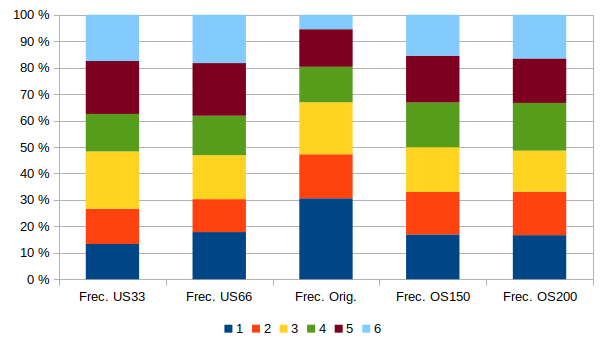
\includegraphics[scale=0.63]{supervised-resample-bias1-dist}
    \caption{Frecuencias de clases al hacer resamples con \code{biasToUniformClass=1}}
    \label{fig:supervised-resample-bias1-dist}
\end{figure}

\subsection{filters/supervised/instance/ClassBalancer}
\label{sec:supervised-class-balancer}
El filtro supervisado \code{ClassBalancer} asigna pesos ponderados a los patrones de manera que se equilibren las clases. Los patrones de una clase menos frecuente tendrán pesos ponderados mayores y viceversa, de manera que cada clase tenga en suma el mismo peso. En caso de que la clase fuese numérica, el filtro además la discretiza.

\begin{figure}[ht]
    \centering
    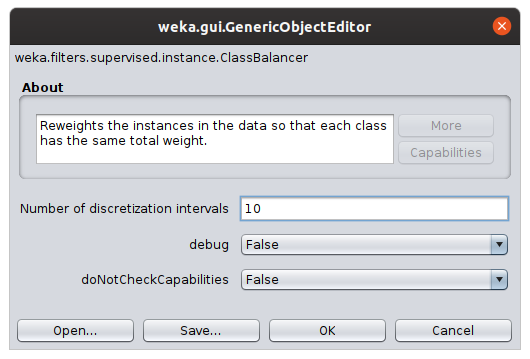
\includegraphics[scale=0.35]{supervised-class-balancer}
    \caption{Diálogo de configuración del filtro supervisado \code{ClassBalancer}}
    \label{fig:supervised-class-balancer}
\end{figure}

Los parámetros del filtro son los que aparecen en la figura \ref{fig:supervised-class-balancer} y se describen a continuación:
\begin{itemize}
    \item \code{Number of discretization intervals (10)}: Nº de intervalos que se establecen al discretizar la clase, en caso de que sea de tipo numérico.
    \item \code{debug False/True}: si se pone a true saca más información en el log al ejecutar el filtro.
    \item \code{doNotCheckCapabilities (False/True)}: habilita o deshabilita la comprobación de los datos. Afecta al rendimiento del filtro.
\end{itemize}

Para probar este filtro se compondrá una base de datos de ejemplo, desbalanceada y con clase continua, de forma que podamos observar a la vez todas las capacidades del filtro. Cuando se aplica el filtro, la primera diferencia que se observa es que el gráfico de distribución de valores de la clase cambia (figs. \ref{fig:supervised-class-balancer-unweighted} y \ref{fig:supervised-class-balancer-weighted}).

\begin{figure}[H]
    \centering
    \begin{minipage}{0.50\textwidth}
        \centering
        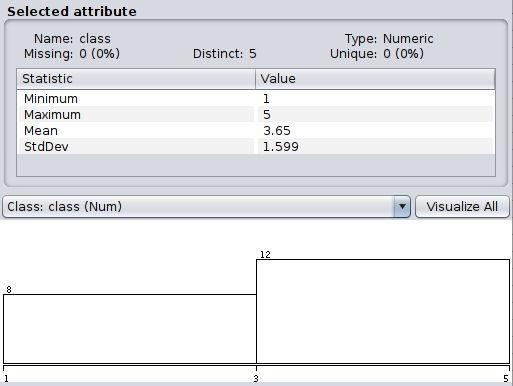
\includegraphics[scale=0.4]{supervised-class-balancer-unweighted}
        \caption{Datos de la clase antes de aplicar el filtro.}
        \label{fig:supervised-class-balancer-unweighted}
    \end{minipage}\hfill
    \begin{minipage}{0.50\textwidth}
        \centering
        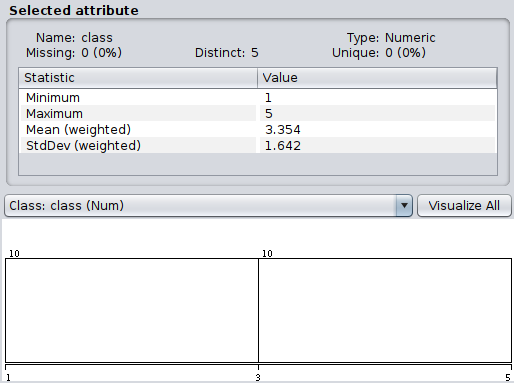
\includegraphics[scale=0.4]{supervised-class-balancer-weighted}
        \caption{Datos de la clase después de aplicar el filtro.}
        \label{fig:supervised-class-balancer-weighted}
    \end{minipage}
\end{figure}

Al aplicar el filtro, se ha añadido un nuevo campo llamado \code{Weight 1} con un valor numérico que representa el peso de la instancia para equilibrar la clase a la que pertenece. En la figura \ref{fig:supervised-class-balancer-int2} podemos ver cómo los pesos asignados balancean la clase en dos intervalos: $[1,3]$ y $(3,5]$. El primer intervalo tiene un peso de $0.8\overline{3}$ y tiene 12 patrones $0.8\overline{3}\cdot 12 = 10$. El segundo intervalo tiene un peso de $1.25$ y contiene 8 patrones: $1.25\cdot 8=10$. En la figura \ref{fig:supervised-class-balancer-int5} podemos ver cómo los pesos asignados balancean la clase en cinco grupos, tantos como valores diferentes toma la clase. A los $3$ patrones clase $1$ se les asigna peso $1.\overline{3}$, por lo que $1.\overline{3}\cdot 3 = 4$. A los 3 patrones con clase 2, les corresponde, obviamente, el mismo peso que a los de clase 1. A los 2 de clase 3, al igual que a los dos de clase 4, se les asigna peso $2$, resultando $2\cdot2=4$. Por último, a los $10$ patrones de clase 5 se les asigna peso $0.4$, lo que resulta en $0.4\cdot10=4$. Como se puede observar, todos los intervalos tienen el mismo peso.

\begin{figure}[H]
    \centering
    \begin{minipage}{0.50\textwidth}
        \centering
        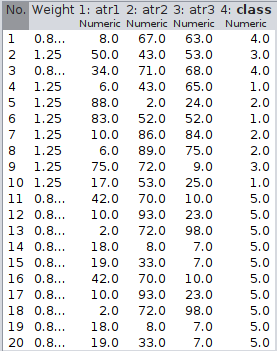
\includegraphics[scale=0.5]{supervised-class-balancer-int2}
        \caption{Datos balanceados en dos intervalos.}
        \label{fig:supervised-class-balancer-int2}
    \end{minipage}\hfill
    \begin{minipage}{0.50\textwidth}
        \centering
        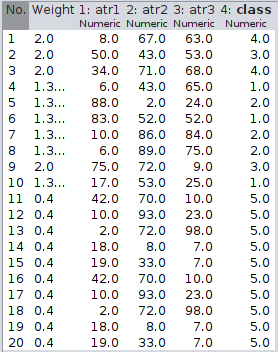
\includegraphics[scale=0.5]{supervised-class-balancer-int5}
        \caption{Datos balanceados en cinco intervalos.}
        \label{fig:supervised-class-balancer-int5}
    \end{minipage}
\end{figure}

\subsection{filters/supervised/instance/SpreadSubsample}
El filtro supervisado \code{SpreadSubsample} realiza remuestreos balanceados de la base de datos. Es decir, produce un nuevo conjunto a partir del anterior con un determinado balance de frecuencias de las clases.


\begin{figure}[H]
    \centering
    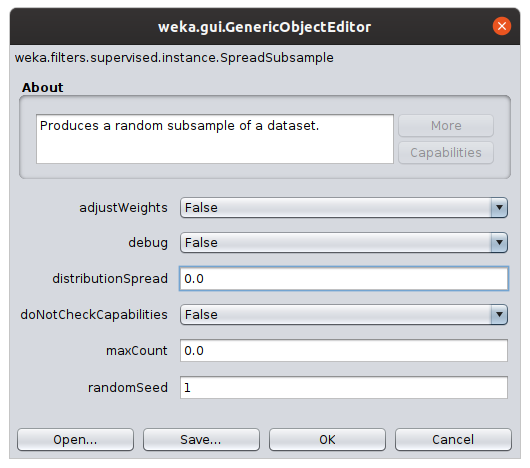
\includegraphics[scale=0.4]{supervised-spread-subsample}
    \caption{Configuración del filtro supervisado \code{SpreadSubsample}.}
    \label{fig:supervised-spread-subsample}
\end{figure}

Como se puede observar en la fig. \ref{fig:supervised-spread-subsample}, el filtro \code{SpreadSubsample} cuenta con los siguientes parámetros:
\begin{itemize}
    \item \code{adjustWeights (False/True)}: si se pone a true, añade a la base de datos el campo \code{Weight} y le asigna un peso ponderado para mantener el mismo equilibro entre clases que hubiera antes de aplicar el filtro (ver \ref{sec:supervised-class-balancer}).
    \item \code{debug (False/True)}: si se pone a true saca más información en el log al ejecutar el filtro.
    \item \code{distributionSpread (num)}: 0 para no establecer proporción máxima, $n | 10\geq n\geq 1$ para permitir un desequilibro máximo entre clases clases de $n:1$.
    \item \code{doNotCheckCapabilities (False/True)}: habilita o deshabilita la comprobación de los datos. Afecta al rendimiento del filtro.
    \item \code{maxCount (num)}: establece un límite máximo de patrones por clase. 0 para desactivar esta función.
    \item \code{randomSeed (num)}: semilla para la selección aleatoria.
\end{itemize}

Para probar este filtro se utiliza la base de datos \code{breast-cancer} por ser su clase binaria y con una distribución 201-85 (fig. \ref{fig:supervised-spread-subsample-breast-cancer}). En una primera prueba, con los parámetros por defecto, no se ha visto ningún cambio en la base de datos al aplicar el filtro. El primer cambio introducido ha sido el valor 50 en el parámetro \code{maxCount}, lo que ha producido subsampling que ha igualado el nº de patrones de cada clase a 50 (fig. \ref{fig:supervised-spread-subsample-max50}).


\begin{figure}[H]
    \centering
    \begin{minipage}{0.50\textwidth}
        \centering
        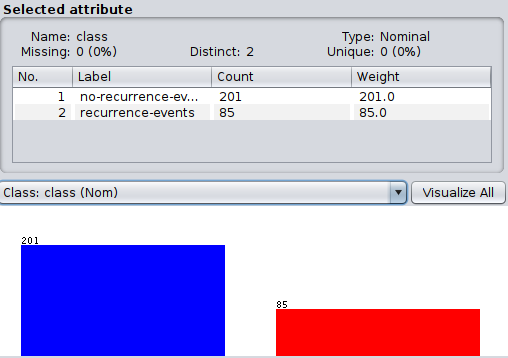
\includegraphics[scale=0.40 ]{supervised-spread-subsample-breast-cancer}
        \caption{Distribución inicial de la clase en la base de datos \code{breast-cancer}.}
        \label{fig:supervised-spread-subsample-breast-cancer}
    \end{minipage}\hfill
    \begin{minipage}{0.50\textwidth}
        \centering
        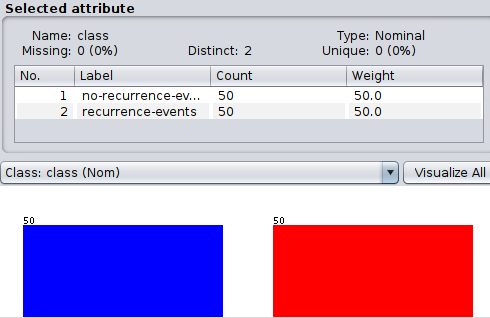
\includegraphics[scale=0.44]{supervised-spread-subsample-max50}
        \caption{Resultado del filtro con distributionSpread=0 y maxCount=50.}
        \label{fig:supervised-spread-subsample-max50}
    \end{minipage}
\end{figure}

La segunda prueba ha consistido en fijar de nuevo \code{maxCount} a 0 y \code{distributionSpread}a 1. Esta configuración sirve para que la proporción máxima entre las clases sea $1:1$, así que también equilibra la distribución de las clases, eliminando patrones de la clase mayoritaria hasta quedar tantos como tenga la minoritaria (fig. \ref{fig:supervised-spread-subsample-spr1}). Por último, se establece \code{distributionSpread} a 1.5 con el fin de obtener una proporción $3:2$. Deberíamos tener 3 patrones de la clase \code{no-recurrence-events} por cada dos de la clase \code{recurrence-events}. Una vez aplicado el filtro con la configuración indicada (fig. \ref{fig:supervised-spread-subsample-spr1.5}), vemos que el resultado es el esperado: 127 frente a 85 patrones de cada clase.

\begin{figure}[H]
    \centering
    \begin{minipage}{0.50\textwidth}
        \centering
        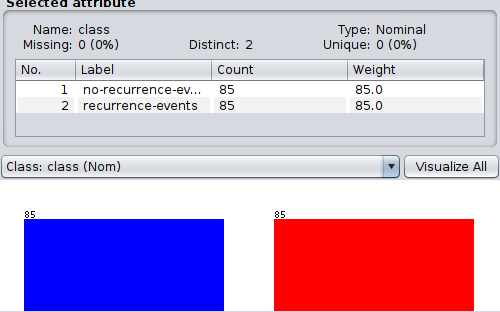
\includegraphics[scale=0.44]{supervised-spread-subsample-spr1}
        \caption{Resultado del filtro con distributionSpread=1 y maxCount=0.}
        \label{fig:supervised-spread-subsample-spr1}
    \end{minipage}\hfill
    \begin{minipage}{0.50\textwidth}
        \centering
        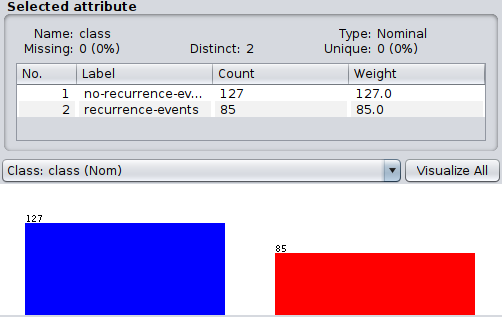
\includegraphics[scale=0.45]{supervised-spread-subsample-spr15}
        \caption{Resultado del filtro con distributionSpread=1.5.}
        \label{fig:supervised-spread-subsample-spr1.5}
    \end{minipage}
\end{figure}
% \part{Práctica 2}
\section{Actividad 2-1}
\label{p21}
\begin{center}
    \parbox{12cm}{\justify\textit{Para esta práctica, utilice el conjunto de datos de altura de ola proporcionado en Moodle.\\
    Describa las operaciones de preprocesamiento que ha realizado sobre la base de datos proporcionada y cómo queda la base de datos final ya preprocesada. Se deja a su elección el conjunto de técnicas a aplicar, así como el nivel de detalle y descripción que quiera dar a su trabajo. \\   
    Para probar rendimientos sobre su preprocesamiento, puede lanzar cualquier algoritmo de Weka, por ejemplo classifiers.functions.Logistic, y fijarse en la métrica ``Correctly Classified Instances''. En la opción ``Suplied test set'' se indicaría el fichero del conjunto de test, mientras que el de entrenamiento corresponde al que se ha cargado desde la pestaña Preprocess.}}
\end{center}

\subsection{Introducción}
En este ejercicio se van a poner en práctica los conceptos aprendidos sobre preprocesamiento de datos. Para ello se utilizará una base de datos de observaciones meteorológicas tomadas entre 2014 y 2016 a razón de 4 mediciones al día. El conjunto tiene 3559 patrones con 17 atributos numéricos y una clase nominal. Los atributos son:
\begin{itemize}
    \item AIR: Temperatura del aire en la superficie (ºK).
    \item PRES: Presión a nivel de superficie (Pa).
    \item RHUM: Humedad relativa a nivel de superficie (\%).
    \item UWND: Velocidad del viento de oeste a este (eje X) (m/s).
    \item VWND: Velocidad del viento de sur a norte (eje Y) (m/s).
    \item WDIR: Dirección del viento en el sentido de las agujas del reloj (grad).
    \item WSPD: Velocidad del viento (m/s).
    \item GST: Velocidad de pico del viento (m/s).
    \item DPD: Periodo de ola dominante (s).
    \item APD: Periodo medio de ol a dominante (s).
    \item MWD: Dirección de la que viene el periodo de ola dominante (grad).
    \item PRES: Presión a nivel de superficie (HPa).
    \item ATMP: Temperatura del aire en la parte superior de la boya (ºC).
    \item WTMP: Temperatura a nivel del mar (ºC).
    \item DEWP: Punto de rocío tomado a la misma altura que ATMP (ºC).
    \item VIS: Visibilidad desde la boya (MN).
    \item TIDE: NIvel del agua por encima o por debajo de la media inferior del agua (Pies).
\end{itemize}
La variable de salida indica la altura de ola en las seis horas siguientes. Es discreta con valores Baja, Media, Moderada y MuyAlta.

Para valorar el preprocesamiento realizado, se generará a cada paso un clasificador logístico y se evaluará con un conjunto de pruebas con la misma estructura que contiene los datos correspondientes a los años 2017 y 2018. Este proceso se realiza desde la pestaña Classify de Weka Explorer. El clasificador seleccionado será Functions.Logistic con la configuración indicada en la figura \ref{fig:classifiers-functions-logistic-config} y utilizando como conjunto de test el archivo \code{alturaolatest.arff}, al que previamente se le habrá realizado el correspondiente tratamiento.

\begin{figure}[ht]
    \centering
    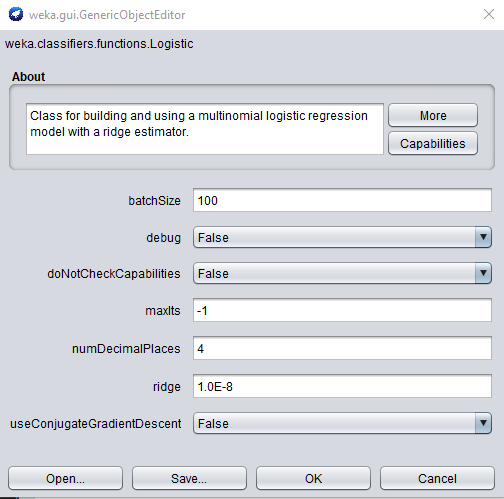
\includegraphics[scale=0.4]{classifiers-functions-logistic-config}
    \caption{Configuración del clasificador logístico}
    \label{fig:classifiers-functions-logistic-config}
\end{figure}

\subsection{Preparación}
Como paso previo se han convertido los archivos \code{.csv} a \code{.arff}. Los dos archivos se han cargado en Weka para poder visualizar su contenido, como puede verse en las figuras \ref{fig:altura-ola-orig} y \ref{fig:altura-ola-test-orig}.

\begin{figure}[H]
    \centering
    \begin{minipage}{0.5\textwidth}
        \centering
        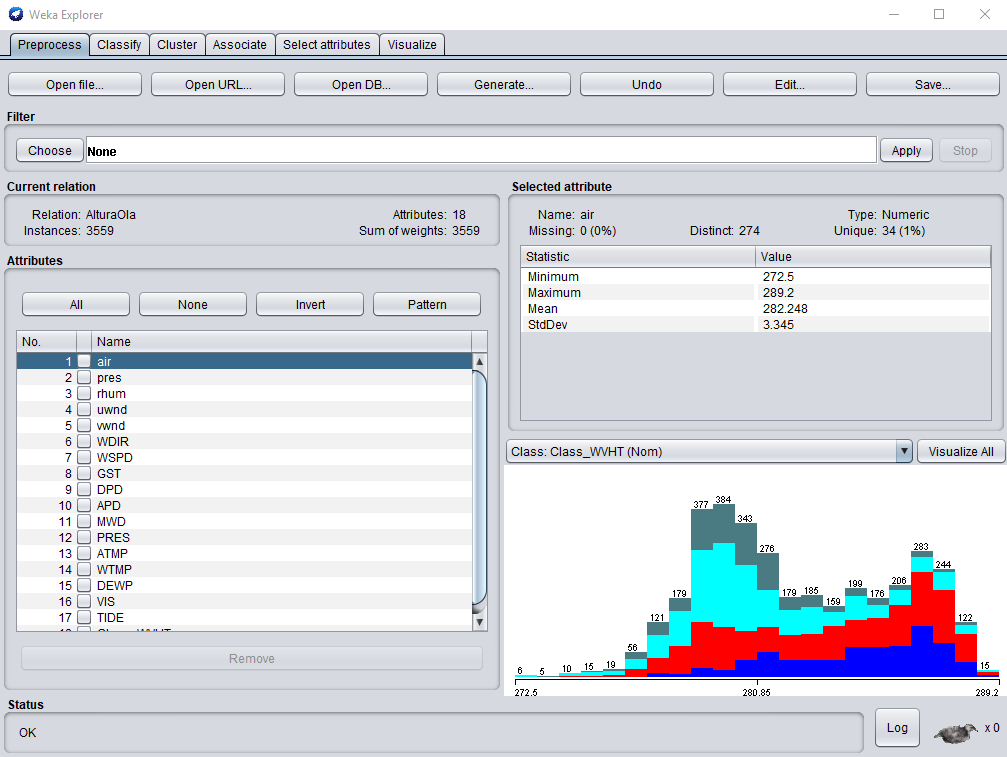
\includegraphics[scale=0.29]{altura-ola-orig}
        \caption{Captura de \code{alturaola.arff}.}
        \label{fig:altura-ola-orig}
    \end{minipage}\hfill
    \begin{minipage}{0.5\textwidth}
        \centering
        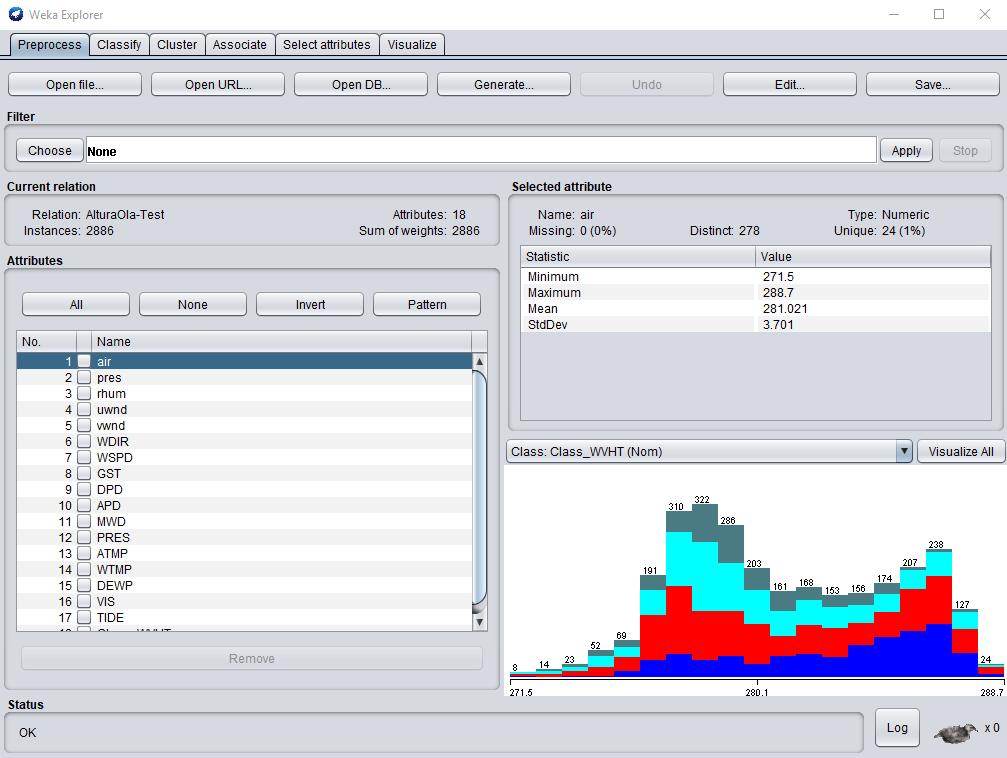
\includegraphics[scale=0.29]{altura-ola-test-orig}
        \caption{Captura de \code{alturaolatest.arff}.}
        \label{fig:altura-ola-test-orig}
    \end{minipage}
\end{figure}

Tras la conversión de los archivos y antes de empezar el tratamiento de los datos, se ha generado y testeado el clasificador logístico para ver el punto de partida. En la figura \ref{fig:clasificador-logistico-resultados-00} se pueden observar los resultados: se tiene en el punto de partida un $71.9335\%$ de patrones correctamente clasificados y precisión mínima de $0.660$ para la clase ``Media''.

\begin{figure}[ht]
    \centering
    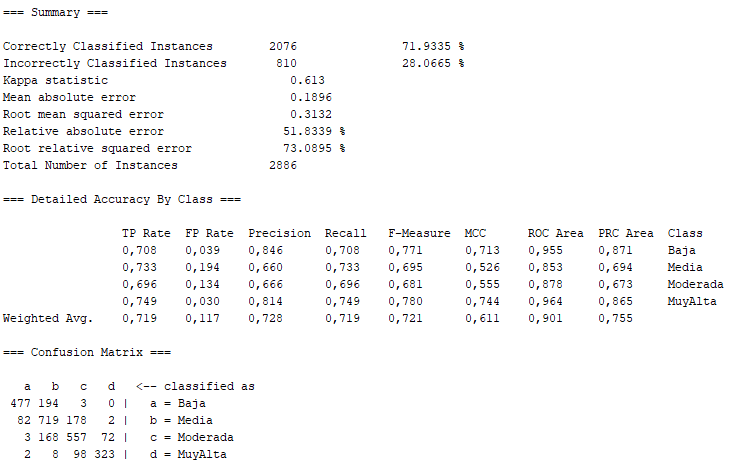
\includegraphics[scale=0.8]{clasificador-logistico-resultados-00}
    \caption{Resultados del clasificador logístico antes del tratamiento de datos.}
    \label{fig:clasificador-logistico-resultados-00}
\end{figure}

\subsection{Datos perdidos}
En primer lugar se eliminan los tres atributos con 100\% de datos perdidos: TIDS, VIS y MWD tanto en el conjunto de entrenamiento como en el de test y se genera de nuevo el clasificador logístico. Como se puede observar en la figura \ref{fig:clasificador-logistico-resultados-01}, la eliminación de los atributos con 100\% de datos perdidos no tiene ningún efecto.

\begin{figure}[ht]
    \centering
    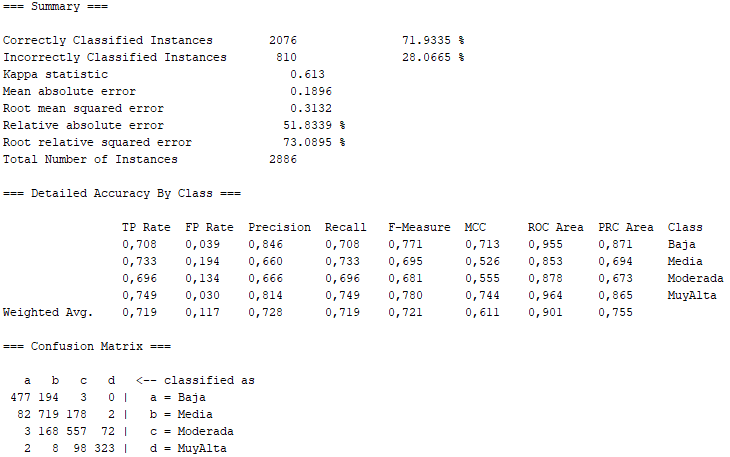
\includegraphics[trim={0cm 10.4cm 7cm 0.7cm},clip]{clasificador-logistico-resultados-01}
    \caption{Resultados tras eliminar TIDS, VIS y MWD.}
    \label{fig:clasificador-logistico-resultados-01}
\end{figure}
% Datos en alturaola.02.datos-perdidos-a.arff y alturaolatest.02-datos-perdidos-a.arff

A continuación se estudian los campos con valores perdidos que son en entrenamiento DPD, APD, PRES y DEWP con 8 (<1\%), 8 (<1\%), 553 (16\%) y 1189 (33\%) patrones con datos perdidos respectivamente y en pruebas WSPD, GST, DPD, APD, PRES, ATMP, WTMP Y DEWP. Para estos casos se reemplazan los valores perdidos por la media de la clase calculada sobre el conjunto de entrenamiento tanto en el conjunto de entrenamiento como en el conjunto de generalización (ver cuadro \ref{tab:medias-por-clase}). Se realiza este procedimiento siguiendo el consejo del archivo \code{Imputación de valores perdidos mas justa en training y test.pdf}, aunque me preocupa en qué medida contribuirá al rendimiento del modelo cuando se exponga a datos nuevos.

\begin{table}[ht]
    \centering
    \begin{tabular}{|r|rlrl|rrrr|}
    \hline
      \multicolumn{1}{|c|}{} &
      \multicolumn{4}{c|}{Datos perdidos} &
      \multicolumn{4}{c|}{Medias en entrenamiento} \\
      \multicolumn{1}{|c|}{Atributo} &
      \multicolumn{2}{c}{Entrenamiento} &
      \multicolumn{2}{c|}{Test} &
      \multicolumn{1}{c}{Baja} &
      \multicolumn{1}{c}{Media} &
      \multicolumn{1}{c}{Moderada} &
      \multicolumn{1}{c|}{MuyAlta} \\ \hline
      WSPD & 0    & (0\%)  & 1    & (<1\%)  & 4,6    & 6,6    & 8,4    & 11,9   \\ 
      GST  & 0    & (0\%)  & 9    & (<1\%)  & 5,6    & 8,1    & 10,5   & 14,9   \\
      DPD  & 8    & (<1\%) & 21   & (1\%)   & 11,5   & 10,3   & 10,8   & 11,7   \\
      APD  & 8    & (<1\%) & 21   & (1\%)   & 6,5    & 6,7    & 7,0    & 7,7    \\
      PRES & 553  & (16\%) & 6    & (<1\%)  & 1017,8 & 1013,1 & 1008,7 & 1007,2 \\
      ATMP & 0    & (0\%)  & 3    & (<1\%)  & 11,5   & 9,9    & 7,8    & 7,4    \\
      WTMP & 0    & (0\%)  & 7    & (<1\%)  & 12,3   & 10,8   & 8,8    & 8,2    \\
      DEWP & 1189 & (33\%) & 2886 & (100\%) & 8,9    & 7,1    & 4,8    & 4,8    \\\hline
    \end{tabular}
    \caption{Datos perdidos y medias de atributos en entrenamiento por clase.}
    \label{tab:medias-por-clase}
\end{table}

Una vez reemplazados todos los datos perdidos se obtienen en el clasificador los resultados mostrados en la figura \ref{fig:clasificador-logistico-resultados-02b}, en los que se observa una mejora en las métricas del clasificador. Por ejemplo, el CCR sube casi un 3\%, la mínima sensibilidad aumenta ligeramente y el área bajo la curva ROC aumenta para tres de las cuatro clases.
% Datos en alturaola.02.datos-perdidos-b.arff y alturaolatest.02-datos-perdidos-b.arff

\begin{figure}[ht]
    \centering
    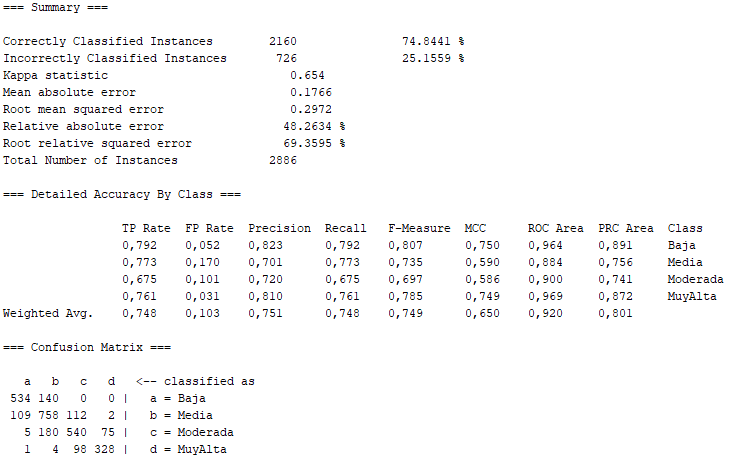
\includegraphics[scale=0.8]{clasificador-logistico-resultados-02}
    \caption{Resultados tras reemplazar los datos perdidos}
    \label{fig:clasificador-logistico-resultados-02b}
\end{figure}

\subsection{Unificación de medidas}
El siguiente paso a seguir será la estandarización de las unidades de medida de los atributos que representan la misma magnitud. En nuestro dataset tenemos dos pares de atributos que representan temperatura y presión respectivamente, y utilizan diferentes unidades (ºC/ºK por un lado y HPas/Pas), por lo que correspondería a unificarlas. Las transformaciones se han realizado mediante el filtro \code{MathExpression}. Primero se han pasado a Pascales los valores del atributo PRES que estaban en HPas y seguidamente se han pasado a ºC los valores del atributo \code{air} que se encontraban en ºK. Como era de esperar, estas operaciones no han tenido ningún efecto sobre el resultado del clasificador.
% Datos en alturaola.03.unidades.arff y alturaolatest.03.unidades.arff

\subsection{Selección de características}
En esta etapa del preprocesamiento vamos a intentar detectar los atributos que influyen muy poco en la clase (atributos irrelevantes) para así eliminarlos y simplificar el modelo. Del mismo modo, intentaremos identificar pares de atributos con una correlación alta (atributos redundantes) para prescindir, de entre los dos, de el que menos influya en la clase.

\subsubsection{Análisis de atributos irrelevantes}
Para medir la influencia de cada atributo sobre la clase del dataset en Weka utilizaremos el evaluador de atributos \code{CorrelationAttributeEval} en combinación con \code{Ranker} como método de búsqueda en la pestaña ``Select attributes'' del explorador de Weka. La salida de este análisis se puede ver en la figura \ref{fig:correlation-attribute-eval}.

\begin{figure}[H]
    \centering
    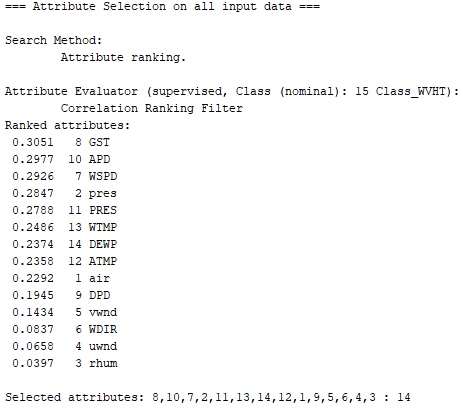
\includegraphics[scale=0.51]{03-correlation-attribute-eval}
    \caption{Resultados de \code{CorrelationAttributeEval}}
    \label{fig:correlation-attribute-eval}
\end{figure}

Lo siguiente será eliminar uno por uno atributos desde el menos influyente (\code{rhum}) hacia arriba comprobando el resultado del clasificador logístico hasta que comience a empeorar. Se eliminan \code{rhum} y \code{uwnd} para alcanzar un $CCR=75,23\%$ (fig. \ref{fig:03-quitar-irrelevantes}), pero al eliminar \code{WDIR} vemos que empeora, por lo que paramos ahí. No estoy seguro de si este paso para reducir la complejidad conviene o no conviene en este caso ya que a pesar de la leve mejora del CCR, vemos en la matriz de confusión que la única clase que ha mejorado en nº de patrones bien clasificados es \code{Media}, que ya era la que mejor clasificaba, a costa de un empeoramiento en el resto. 

\begin{figure}[ht]
    \centering
    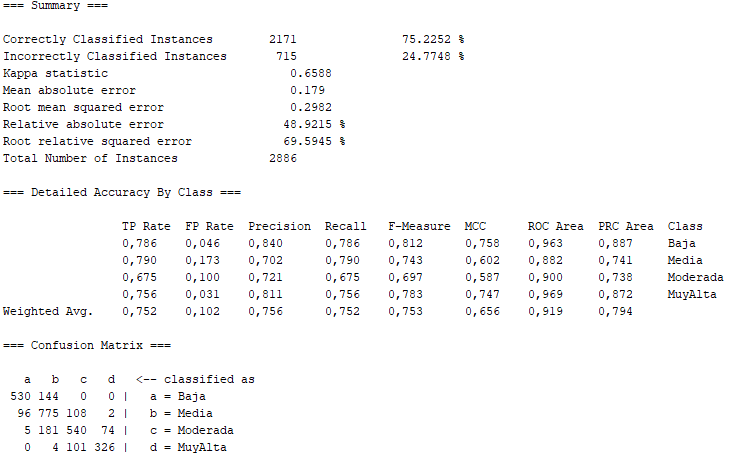
\includegraphics[scale=0.8]{03-quitar-irrelevantes}
    \caption{Resultados tras eliminar atributos irrelevantes}
    \label{fig:03-quitar-irrelevantes}
\end{figure}


\subsubsection{Análisis de atributos redundantes}
A continuación se estudiará la correlación entre atributos. Para realizar este análisis en Weka utilizamos el evaluador de atributos \code{PrincipalComponents} junto con el buscador \code{Ranker}. Podemos ver la tabla de correlaciones obtenida en el cuadro \ref{cuadro:correlaciones}, en el que se han marcado en rojo, naranja y amarillo las correlaciones por encima de 0,6 según su importancia (rojo la más importante). El proceso de eliminación de atributos correlados será el siguiente:
\begin{enumerate}
    \item Elegir un par atributos con correlación alta.
    \item Del par elegido, eliminar el atributo menos correlado con la clase según la figura \ref{fig:correlation-attribute-eval}.
    \item Generar y evaluar el clasificador logístico.
    \begin{enumerate}
        \item Si el resultado mejora, se mantiene la eliminación del atributo.
        \item Si no mejora, se restituye el atributo.
    \end{enumerate}
\end{enumerate}

\begin{table}[ht]
    \resizebox{\textwidth}{!}{%
    \begin{tabular}{|
    >{\columncolor[HTML]{9B9B9B}}c |rrrrrrrrrrrr|}
    \hline
    \cellcolor[HTML]{FFFFFF}{\color[HTML]{FFFFFF} } & \multicolumn{1}{c}{\cellcolor[HTML]{9B9B9B}{\color[HTML]{FFFFFF} air}} & \multicolumn{1}{c}{\cellcolor[HTML]{9B9B9B}{\color[HTML]{FFFFFF} pres}} & \multicolumn{1}{c}{\cellcolor[HTML]{9B9B9B}{\color[HTML]{FFFFFF} vwnd}} & \multicolumn{1}{c}{\cellcolor[HTML]{9B9B9B}{\color[HTML]{FFFFFF} WDIR}} & \multicolumn{1}{c}{\cellcolor[HTML]{9B9B9B}{\color[HTML]{FFFFFF} WSPD}} & \multicolumn{1}{c}{\cellcolor[HTML]{9B9B9B}{\color[HTML]{FFFFFF} GST}} & \multicolumn{1}{c}{\cellcolor[HTML]{9B9B9B}{\color[HTML]{FFFFFF} DPD}} & \multicolumn{1}{c}{\cellcolor[HTML]{9B9B9B}{\color[HTML]{FFFFFF} APD}} & \multicolumn{1}{c}{\cellcolor[HTML]{9B9B9B}{\color[HTML]{FFFFFF} PRES}} & \multicolumn{1}{c}{\cellcolor[HTML]{9B9B9B}{\color[HTML]{FFFFFF} ATMP}} & \multicolumn{1}{c}{\cellcolor[HTML]{9B9B9B}{\color[HTML]{FFFFFF} WTMP}} & \multicolumn{1}{c|}{\cellcolor[HTML]{9B9B9B}{\color[HTML]{FFFFFF} DEWP}} \\ \hline
    {\color[HTML]{FFFFFF} air} & \cellcolor[HTML]{9B9B9B}{\color[HTML]{FFFFFF} 1} & 0,23 & -0 & 0,1 & -0,15 & -0,18 & -0,34 & -0,44 & 0,23 & \cellcolor[HTML]{FE0000}{\color[HTML]{FFFFFF} 0,98} & \cellcolor[HTML]{FE0000}{\color[HTML]{FFFFFF} 0,94} & \cellcolor[HTML]{F8A102}{\color[HTML]{FFFFFF} 0,77} \\
    {\color[HTML]{FFFFFF} pres} & 0,23 & \cellcolor[HTML]{9B9B9B}{\color[HTML]{FFFFFF} 1} & -0,2 & 0,25 & -0,34 & -0,37 & -0,26 & -0,43 & \cellcolor[HTML]{FE0000}{\color[HTML]{FFFFFF} 0,95} & 0,26 & 0,26 & 0,22 \\
    {\color[HTML]{FFFFFF} vwnd} & -0 & -0,2 & \cellcolor[HTML]{9B9B9B}{\color[HTML]{FFFFFF} 1} & -0,15 & 0,31 & 0,31 & 0,07 & 0,13 & -0,2 & -0,01 & -0,12 & 0,08 \\
    {\color[HTML]{FFFFFF} WDIR} & 0,1 & 0,25 & -0,15 & \cellcolor[HTML]{9B9B9B}{\color[HTML]{FFFFFF} 1} & -0,06 & -0,07 & -0,04 & -0,09 & 0,17 & 0,14 & 0,2 & 0,05 \\
    {\color[HTML]{FFFFFF} WSPD} & -0,15 & -0,34 & 0,31 & -0,06 & \cellcolor[HTML]{9B9B9B}{\color[HTML]{FFFFFF} 1} & \cellcolor[HTML]{FE0000}{\color[HTML]{FFFFFF} 0,99} & 0,02 & 0,1 & -0,34 & -0,17 & -0,21 & -0,18 \\
    {\color[HTML]{FFFFFF} GST} & -0,18 & -0,37 & 0,31 & -0,07 & \cellcolor[HTML]{FE0000}{\color[HTML]{FFFFFF} 0,99} & \cellcolor[HTML]{9B9B9B}{\color[HTML]{FFFFFF} 1} & 0,04 & 0,14 & -0,36 & -0,2 & -0,23 & -0,21 \\
    {\color[HTML]{FFFFFF} DPD} & -0,34 & -0,26 & 0,07 & -0,04 & 0,02 & 0,04 & \cellcolor[HTML]{9B9B9B}{\color[HTML]{FFFFFF} 1} & \cellcolor[HTML]{F8A102}{\color[HTML]{FFFFFF} 0,71} & -0,27 & -0,33 & -0,31 & -0,3 \\
    {\color[HTML]{FFFFFF} APD} & -0,44 & -0,43 & 0,13 & -0,09 & 0,1 & 0,14 & \cellcolor[HTML]{F8A102}{\color[HTML]{FFFFFF} 0,71} & \cellcolor[HTML]{9B9B9B}{\color[HTML]{FFFFFF} 1} & -0,45 & -0,44 & -0,44 & -0,41 \\
    {\color[HTML]{FFFFFF} PRES} & 0,23 & \cellcolor[HTML]{FE0000}{\color[HTML]{FFFFFF} 0,95} & -0,2 & 0,17 & -0,34 & -0,36 & -0,27 & -0,45 & \cellcolor[HTML]{9B9B9B}{\color[HTML]{FFFFFF} 1} & 0,24 & 0,25 & 0,2 \\
    {\color[HTML]{FFFFFF} ATMP} & \cellcolor[HTML]{FE0000}{\color[HTML]{FFFFFF} 0,98} & 0,26 & -0,01 & 0,14 & -0,17 & -0,2 & -0,33 & -0,44 & 0,24 & \cellcolor[HTML]{9B9B9B}{\color[HTML]{FFFFFF} 1} & \cellcolor[HTML]{FE0000}{\color[HTML]{FFFFFF} 0,95} & \cellcolor[HTML]{F8A102}{\color[HTML]{FFFFFF} 0,76} \\
    {\color[HTML]{FFFFFF} WTMP} & \cellcolor[HTML]{FE0000}{\color[HTML]{FFFFFF} 0,94} & 0,26 & -0,12 & 0,2 & -0,21 & -0,23 & -0,31 & -0,44 & 0,25 & \cellcolor[HTML]{FE0000}{\color[HTML]{FFFFFF} 0,95} & \cellcolor[HTML]{9B9B9B}{\color[HTML]{FFFFFF} 1} & \cellcolor[HTML]{FFC702}0,66 \\
    {\color[HTML]{FFFFFF} DEWP} & \cellcolor[HTML]{F8A102}{\color[HTML]{FFFFFF} 0,77} & 0,22 & 0,08 & 0,05 & -0,18 & -0,21 & -0,3 & -0,41 & 0,2 & \cellcolor[HTML]{F8A102}{\color[HTML]{FFFFFF} 0,76} & \cellcolor[HTML]{FFC702}0,66 & \cellcolor[HTML]{9B9B9B}{\color[HTML]{FFFFFF} 1} \\ \hline
    \end{tabular}%
    }
    \caption{Correlaciones entre atributos}
    \label{cuadro:correlaciones}
\end{table}
El primer par procesado ha sido \code{pres-PRES} porque tiene una altísima correlación y no es de los atributos más influyentes sobre la clase, pero principalmente porque representan la misma magnitud. Tras la eliminación de \code{PRES}, el clasificador apenas cambia. Sólo mejora muy ligeramente, lo que nos da una idea de lo poco que servía el atributo eliminado, ganando el modelo en simplicidad.

El segundo par procesado ha sido \code{WSPD-GST} por tener la más alta correlación. De los dos atributos, se ha eliminado WSPD por ser el que menos influye sobre la clase. Tras la eliminación, el clasificador apenas ha cambiado. Sólo 8 patrones correctamente clasificados menos, lo que nos lleva a un CCR de $75,09\%$ con una sensibilidad mínima de $0,679$ para la clase <<Moderada>>.

La siguiente correlación más alta se da entre el par \code{air-ATMP}. \code{air} está fuertemente correlacionado con \code{WTMP} y \code{DEWP} también, y al mismo tiempo es el menos correlacionado con la clase de los cuatro, por lo que se va a eliminar. Tras la eliminación vemos que los estadísticos se ven muy poco afectados: $CCR=75,05\%$ y sensibilidad mínima de $0,686$ para la clase <<Moderada>>.

El par \code{WTMP-ATMP} es el siguiente más correlacionado. Como \code{ATMP} es el atributo que menos influye sobre la clase, se elimina éste. El clasificador empeora significativamente pasando a un $CCR=74,22\%$ por lo que se decide no mantener esta eliminación. La eliminación de \code{WTMP} produce un efecto similar ($CCR=74,64\%$), por lo tanto se mantendrán estos dos atributos.

El siguiente par estudiado ha sido \code{APD-DPD}, ya con correlación más baja. El atributo \code{DPD} es mucho menos influyente en la clase, por lo que se decide eliminarlo consiguiendo un ligero aumento de rendimiento en el porcentaje de patrones bien clasificados ($CCR=75,16\%$) así como en la sensibilidad mínima ($0,690$).

El último par es \code{DEWP-WTMP}. \code{DEWP} influye menos en la clase y además, ya se comprobó la influencia negativa de la eliminación de \code{WTMP} en el rendimiento del clasificador, por lo que se elimina \code{DEWP}. Esta eliminación ha tenido un impacto muy negativo sobre el clasificador $CCR=71,86\%$. Por este motivo, la eliminación se revierte y no se eliminan más atributos.

En resumen, se han eliminado los atributos \code{pres}, \code{WSPD}, \code{air} y \code{DPD} reduciendo la complejidad del modelo. Al mismo tiempo, los indicadores del modelo como CCR y mínima sensibilidad han mejorado, alcanzando valores $75,16\%$ y $0,690$ respectivamente (ver figura \ref{fig:clasificador-logistico-resultados-04}).

\begin{figure}[ht]
    \centering
    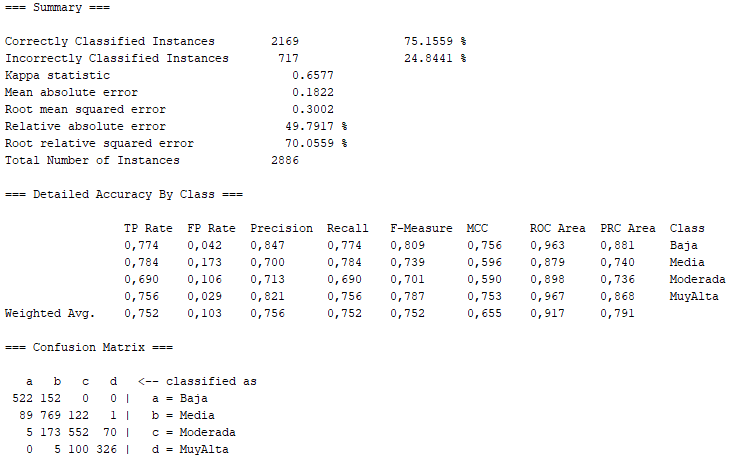
\includegraphics[scale=0.8]{clasificador-logistico-resultados-04}
    \caption{Resultados tras quitar atributos redundantes}
    \label{fig:clasificador-logistico-resultados-04}
\end{figure}


\subsection{Normalización}
El siguiente paso del preprocesamiento consiste en normalizar los datos tanto de entrenamiento como de generalización. Queremos llevar cada atributo a un rango $[0-1]$ en entrenamiento y luego aplicar la misma transformación al conjunto de generalización. Para ello, aplicaremos la fórmula \ref{formula:normalizacion} a cada atributo de ambos conjuntos pero utilizando siempre los máximos y mínimos del conjunto de entrenamiento, tal como aparecen en la tabla \ref{cuadro:maximos-minimos-normalizacion}. El proceso se realizará mediante el filtro \code{MathExpression}, campo a campo. Para el conjunto de entrenamiento se obtiene el mismo resultado utilizando el filtro \code{Normalize}.
\begin{equation} \label{formula:normalizacion}
    a^*=\frac{a-a_{min}}{a_{max}-a_{min}}
\end{equation}

\begin{table}[ht]
    \centering
    \begin{tabular}{|r|r|r|r|r|r|r|r|}
    \hline
    \rowcolor[HTML]{9B9B9B} 
    {\color[HTML]{FFFFFF} } & \multicolumn{1}{c|}{\cellcolor[HTML]{9B9B9B}{\color[HTML]{FFFFFF} pres}} & \multicolumn{1}{c|}{\cellcolor[HTML]{9B9B9B}{\color[HTML]{FFFFFF} vwnd}} & \multicolumn{1}{c|}{\cellcolor[HTML]{9B9B9B}{\color[HTML]{FFFFFF} WDIR}} & \multicolumn{1}{c|}{\cellcolor[HTML]{9B9B9B}{\color[HTML]{FFFFFF} GST}} & \multicolumn{1}{c|}{\cellcolor[HTML]{9B9B9B}{\color[HTML]{FFFFFF} APD}} & \multicolumn{1}{c|}{\cellcolor[HTML]{9B9B9B}{\color[HTML]{FFFFFF} ATMP}} & \multicolumn{1}{c|}{\cellcolor[HTML]{9B9B9B}{\color[HTML]{FFFFFF} WTMP}} \\ \hline
    \cellcolor[HTML]{9B9B9B}{\color[HTML]{FFFFFF} min} & 96020 & -17,9 & 0 & 0,4 & 3,10 & -0,9 & 6 \\ \cline{1-1}
    \cellcolor[HTML]{9B9B9B}{\color[HTML]{FFFFFF} max} & 103850 & 21,1 & 359 & 26,1 & 11,09 & 15,8 & 16,1 \\ \cline{1-1}
    \cellcolor[HTML]{9B9B9B}{\color[HTML]{FFFFFF} ran} & 7830 & 39,0 & 359 & 25,7 & 7,99 & 16,7 & 10,1 \\ \hline
    \end{tabular}
    \caption{Valores máximos, mínimos y rangos por atributo.}
    \label{cuadro:maximos-minimos-normalizacion}
\end{table}

Como se puede comprobar en la figura \ref{fig:clasificador-logistico-resultados-05}, el proceso de normalización ha provocado un empeoramiento generalizado del rendimiento del clasificador, con casi un 4\% menos de patrones correctamente clasificados. No tengo claro que necesariamente cualquier clasificador deba ser mejor con datos normalizados. A la vista de que el clasificador logístico que estamos utilizando para evaluar los efectos del preprocesamiento no se ve beneficiado por la normalización de nuestro conjunto de datos, continúo con los datos sin normalizar.

\begin{figure}[ht]
    \centering
    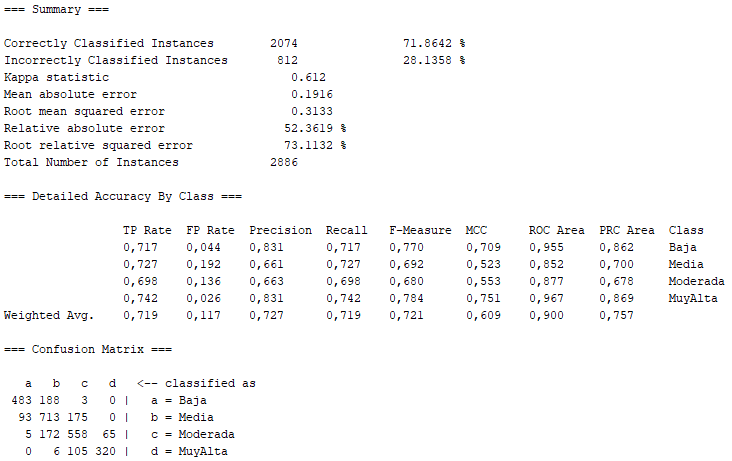
\includegraphics[scale=0.8]{clasificador-logistico-resultados-05}
    \caption{Resultados tras normalización de datos}
    \label{fig:clasificador-logistico-resultados-05}
\end{figure}

\subsection{Datos extremos}
Para la detección de valores extremos, haremos uso del filtro \code{InterquartileRange}. Este filtro añade a la base de datos un par de atributos para indicar si el patrón es un dato extremo o atípico (outlier). Según las transparencias, se consideran valores extremos aquellos que estén a más del doble del rango intercuartílico por debajo del cuartil 1 o por encima del cuartil 3. Aplicando la configuración correspondiente al filtro de Weka, podemos ver que aparecen 33 patrones con datos extremos tal como se muestra en la figura \ref{fig:valores-extremos}.
\begin{figure}[ht]
    \centering
    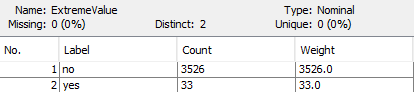
\includegraphics[scale=1]{valores-extremos}
    \caption{Detección de valores extremos con Weka}
    \label{fig:valores-extremos}
\end{figure}
A continuación eliminaremos los patrones con \code{ExtremeValue=yes} utilizando el filtro \code{RemoveWithValues} y posteriormente eliminaremos el atributo \code{ExtremeValues} para poder ejecutar el clasificador logístico con el conjunto de generalización. En dicha ejecución se han obtenido los valores que aparecen en la figura \ref{fig:clasificador-logistico-resultados-06}.

\begin{figure}[H]
    \centering
    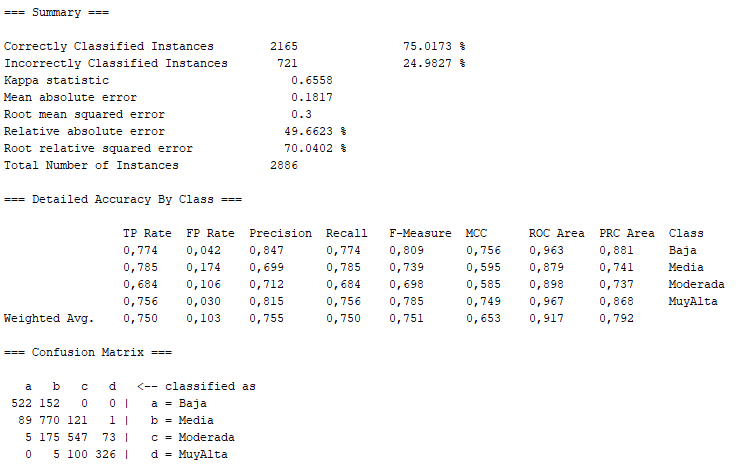
\includegraphics[scale=0.8]{clasificador-logistico-resultados-06}
    \caption{Resultados tras eliminación de valores extremos}
    \label{fig:clasificador-logistico-resultados-06}
\end{figure}

De nuevo observamos un ligero empeoramiento respecto a los resultados de partida (ver fig. \ref{fig:clasificador-logistico-resultados-04}), por lo que no parece conveniente, en este caso, eliminar los valores extremos. Esto parece lógico ya que también hay valores de este tipo en el conjunto de test, y si el modelo no los aprende, difícilmente podrá luego clasificarlos en generalización.
% \part{Práctica 3}
\section{Actividad 3-1}
\label{p31}
\begin{center}
    \parbox{12cm}{\justify\textit{Escoja una de las bases de datos de clasificación para el trabajo de las dispuestas en Moodle (Breast Cancer, Dermatology, Fantasmas, Glass, Vehicle, Wine, Zoo). \\
    Se entiende que además de pasarla a formato .arff ya ha aplicado el preprocesamiento necesario en función del fichero ``\textbf{Pistas sobre los datasets con posible preprocesamiento a simple vista.pdf}'', en el caso de que sea una de las bases de datos que lo requiera.\\
    Aplique el preprocesamiento adicional (si se puede aplicar sobre: 1) reemplazamiento de datos perdidos, 2) normalización y 3) paso de nominal a binario u ordinar a numérico. \\
    Explique el preprocesamiento que haya llevado a cabo en los aspectos citados, y de no tener que hacerlo explique también por qué.}}
\end{center}

%-------------------------------------------------------------------------------
%-------------------------------------------------------------------------------
%-------------------------------------------------------------------------------
\clearpage
\section{Actividad 3-2}
\label{p32}
\begin{center}
    \parbox{12cm}{\justify\textit{Con la base de datos escogida anteriormente, use el algoritmo de clasificación \textbf{KNN} (IBK en Weka) con un 10-fold crossvalidation. Use un valor de vecinos $k=3$ dejando por defecto el resto de parámetros.\\
    Interprete la salida en cuanto a los valores de las métricas que proporciona Weka.\\
    Tenga en cuenta si se clasifican bien todas las clases de su problema (TP Rate por clase) y fíjese también en la matriz de confusión. \\
    Para explicar los resultados, haga uso de tablas donde se muestren los valores que está interpretando.}}
\end{center}

%-------------------------------------------------------------------------------
%-------------------------------------------------------------------------------
%-------------------------------------------------------------------------------
\clearpage
\section{Actividad 3-3}
\label{p33}
\begin{center}
    \parbox{12cm}{\justify\textit{Con la base de datos escogida anteriormente, ejecute el algoritmo Simple-Logistic con 10-fold crossvalidation. \\
    Analice los modelos obtenidos, las variables que podrían ser más influyentes (valores $\beta$) variables que no se usan y métricas. \\
    Use tablas para explicar los resultados de manera que haya una lectura legible.}}
\end{center}
% \part{Práctica 4}
\section{Actividad 4-1}
\label{p41}
\begin{center}
    \parbox{12cm}{\justify\textit{Escoja una de las bases de datos de clasificación para el trabajo de las dispuestas en Moodle (Breast Cancer, Dermatology, Fantasmas, Glass, Vehicle, Wine, Zoo). \\
    Se entiende que además de pasarla a formato .arff ya ha aplicado el preprocesamiento necesario en función del fichero ``\textbf{Pistas sobre los datasets con posible preprocesamiento a simple vista.pdf}'', en el caso de que sea una de las bases de datos que lo requiera.
    \begin{itemize}
        \item Cargue la base de datos y ejecute el algoritmo \textbf{C4.5} usando un 75\% para entrenar y un 25\% para generalizar, con los parámetros por defecto.
        \item Analice y muestre el árbol obtenido con los parámetros por defecto: nodo principal, número de nodos u hojas, variables presentes y omitidas. Comente también los resultados de las métricas obtenidas.
    \end{itemize}
    }}
\end{center}

Para la realización de esta actividad se va a utilizar la misma base de datos preprocesada de la práctica 3 (fantasmas). El objetivo es construir en Weka un árbol de decisión mediante el algoritmo C4.5, para lo cuál utilizaremos el clasificador llamado ``J48'' en Weka. Tal como indica el enunciado, se divide el conjunto en dos, seleccionando un 75\% (278 patrones) para la construcción del árbol (train) y el 25\%restante (93 patrones) para generalización (test). Weka realiza esta división manteniendo idénticas frecuencias de las clases en cada subconjunto.

El algoritmo construye el árbol mediante un proceso recursivo en el que, para establecer cada nodo se busca el atributo con mayor porcentaje de ganancia de información ($I(C,X_i)/H(X_i)$), generando una partición en dos del conjunto de datos. En caso de que el atributo sea continuo, el algoritmo es capaz de determinar el mejor umbral. Para cada división del conjunto se añade una arista desde el nodo generado y se repite el proceso con el subconjunto correspondiente. Cuando todos los patrones asociados aun determinado recorrido en profundidad tienen la misma clase, se añade un nodo hoja. El algoritmo C4.5 también permite realizar podas que o bien sustituyen un sub-árbol por un nodo hoja o bien por una parte éste (elevación de sub-árbol). Es interesante mencionar que con este algoritmo, a diferencia de C3, sí que podemos encontrar varias veces el mismo atributo al realizar un recorrido del árbol en profundidad, al menos en el caso de atributos continuos y con diferentes umbrales.

Tal como podemos observar en la figura \ref{fig:j48-arbol}, en este caso de estudio, el atributo de mayor ganancia es hair\_length, por tanto se establece como nodo raíz. El árbol generado cuenta con 53 nodos, 27 de los cuáles son nodos hoja. Cada nodo hoja indica la cantidad de patrones que, siendo de la clase indicada, han alcanzado el nodo así como la cantidad de patrones de otras clases que lo han alcanzado, en caso de haber alguno. Los nodos hoja muestran los resultados para todos los patrones, tanto de generalización como de entrenamiento.

\begin{landscape}
    \begin{figure}[H]
        \centering
        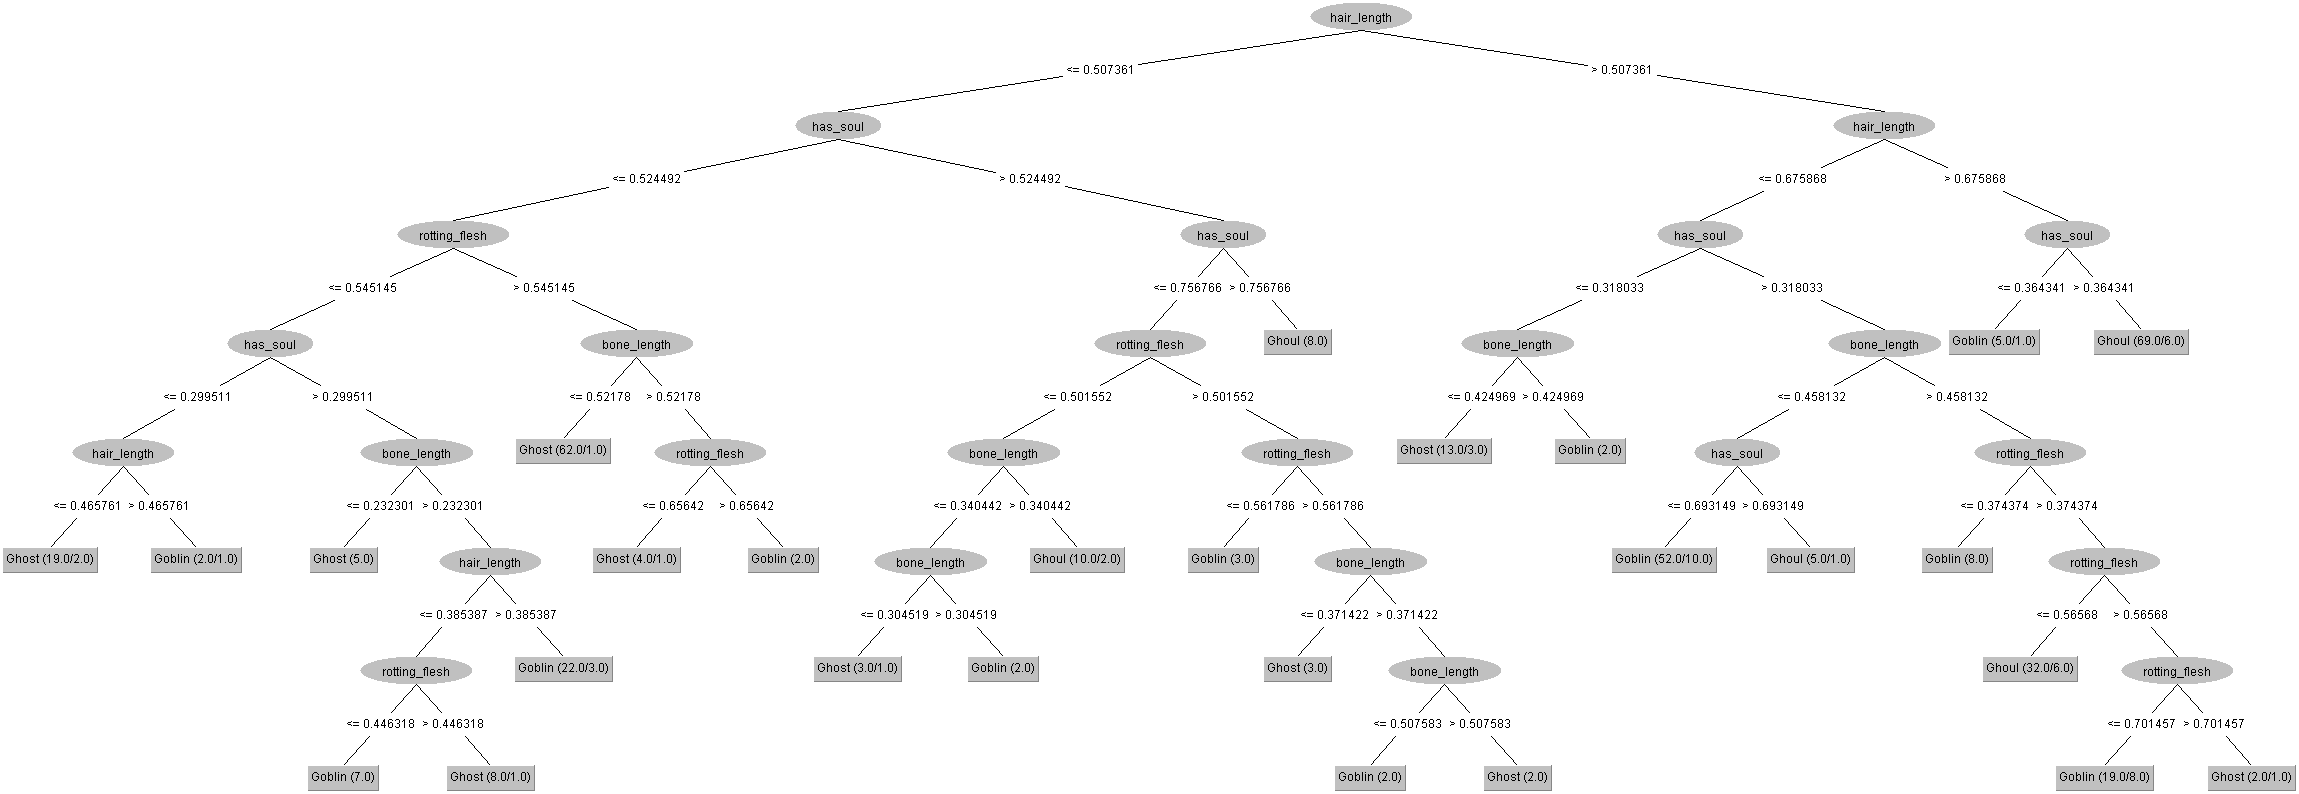
\includegraphics[height=0.5\textheight]{arbol}
        \caption{Árbol de decisión obtenido mediante C4.5}
        \label{fig:j48-arbol}
    \end{figure}
\end{landscape}

De los resultados del clasificador (fig. \ref{fig:j48-resultados}) podemos comentar que se han clasificado correctamente 65 patrones (69,89\%) de un total de 93 del conjunto de generalización. El estadístico Kappa es $\kappa=0,5473$, comparable aunque peor que el obtenido en los ensayos con otros tipos de clasificadores para el mismo conjunto de datos. La clase que peor se reconoce es de nuevo Goblin, con un TP Rate de 0,618, más elevado que el obtenido en los clasificadores anteriores, aunque hay que observar que en este caso, el FP Rate también es más alto, lo que da el peor resultado en AUC para todos los clasificadores utilizados con este conjunto. Esta comparación no es del todo justa porque se ha utilizado una técnica distinta para la generalización. En la matriz de confusión podemos ver que sólo 21 de los 34 Goblins han sido correctamente clasificados.
    
\begin{figure}[H]
    \centering
    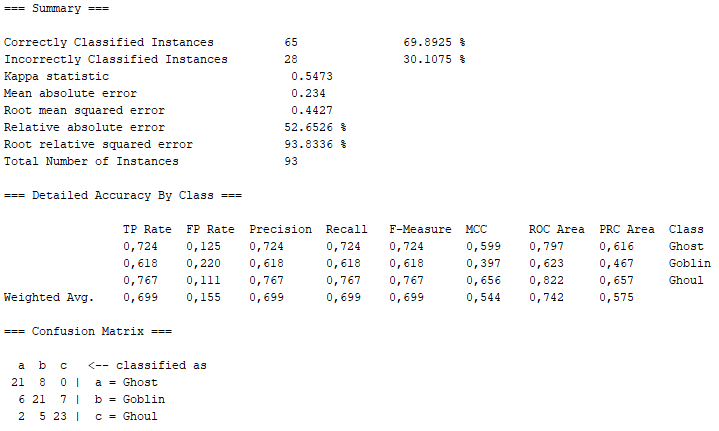
\includegraphics[width=\textwidth,keepaspectratio=true]{j48-resultados}
    \caption{Resultados del clasificador }
    \label{fig:j48-resultados}
\end{figure}


\clearpage
\section{Actividad 4-2}
\label{p42}
\begin{center}
    \parbox{12cm}{\justify\textit{Escoja una de las bases de datos de clasificación para el trabajo de las dispuestas en Moodle (Breast Cancer, Dermatology, Fantasmas, Glass, Vehicle, Wine, Zoo). \\
    Se entiende que además de pasarla a formato .arff ya ha aplicado el preprocesamiento necesario en función del fichero ``\textbf{Pistas sobre los datasets con posible preprocesamiento a simple vista.pdf}'', en el caso de que sea una de las bases de datos que lo requiera.
    \begin{itemize}
        \item Cargue la base de datos con un 75/25\% y ejecute el algoritmo Multilayer-Perceptron con los valores por defecto.
        \item ¿Qué observa al ir modificando sólo el \textbf{TrainingTime}? ¿Cambia el valor de Correctly Classified instances al modificar el parámetro? ¿Se estanca el aprendizaje o sobreentrena?
        \item ¿Qué observa al ir modificando sólo el \textbf{LearningRate}? ¿Cambia el valor de Correctly Classified instances al modificar el parámetro? ¿Se estanca el aprendizaje o sobreentrena?
    \end{itemize}
    }}
\end{center}

Para este ejercicio se utilizará el mismo conjunto de datos preprocesado (fantasmas) que en el ejercicio anterior. La partición del conjunto se realizará al 75/25\% tal como indica el enunciado, por lo que dispondremos de un conjunto de entrenamiento de 278 patrones y un conjunto de generalización de 93 con las mismas frecuencias de clases. El perceptrón tendrá tantos nodos en la capa de entrada como atributos la base de datos y tantos nodos en la capa de salida como valores puede tomar la clase (ver fig. \ref{fig:mlp-red}). Tanto el número de capas ocultas como el número de nodos en cada una de ellas es configurable, como veremos más adelante.

\begin{figure}[ht]
    \centering
    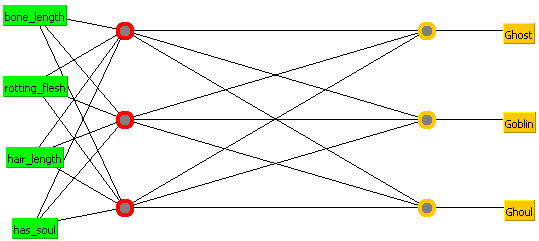
\includegraphics[width=\textwidth,keepaspectratio=true]{mlp-red}
    \caption{Topología de la red}
    \label{fig:mlp-red}
\end{figure}

A continuación repasaremos los parámetros de configuración más importantes y sus valores por defecto\footnote{En la captura se ha modificado el valor de GUI a true para poder capturar el diagrama de la red.} en MultilayerPerceptron (fig. \ref{fig:mlp-configuracion}). 
\begin{itemize}
    \item El parámetro hiddenLayers establece la configuración topológica de la red, en este caso, una única capa oculta con ``a'' nodos, donde el comodín ``a'' toma el valor del punto medio entre el número de atributos independientes y el número de clases. Para nuestro caso, $(3+3/2)=3$ nodos (ver fig. \ref{fig:mlp-red}).
    \item El parámetro learningRate o tasa de aprendizaje indica cuánto se modifican los pesos de las aristas durante el aprendizaje y viene a 0,3.
    \item El parámetro decay a false indica que el factor de aprendizaje se mantendrá constante a lo largo del aprendizaje.
    \item El parámetro momentum representa una especie de inercia que nos permite salir de un mínimo local, y toma valor por defecto 0,2. 
    \item  El parámetro trainingTime indica el número de épocas de entrenamiento, donde una época consiste en la evaluación de un patrón del conjunto de entrenamiento y el posterior ajuste de los pesos de la red mediante back propagation.
    \item El parámetro validationThreshold indica un número de épocas tal que, si el error de validación sube durante más épocas que las indicadas en el umbral, el aprendizaje se para aunque no se haya alcanzado el trainingTime. En el caso por defecto, este umbral se fija a 20 épocas.
\end{itemize}


\begin{figure}[ht]
    \centering
    \includegraphics[width=.5\textwidth,keepaspectratio=true]{mlp-configuracion}
    \caption{Formulario de configuración para MultilayerPerceptron}
    \label{fig:mlp-configuracion}
\end{figure}

Al ejecutar el algoritmo con los valores por defecto, observamos unos resultados (ver fig. \ref{fig:mlp-resultados}) casi idénticos a los que se obtuvieron con J48 (ver fig. \ref{fig:j48-resultados}). $CCR=69,89\%$, 65 patrones correctamente clasificados frente a 28 incorrectamente clasificados, $\kappa=0,5455$, peor TP Rate para la clase Goblin con un valor de 0,676 y 23 goblins correctamente clasificados de 34. Dos más que con J48, aunque hay dos ghouls mal clasificados más y los mismos ghost, de ahí la coincidencia del CCR.


\begin{figure}[H]
    \centering
    \includegraphics[width=\textwidth]{mlp-resultados}
    \caption{Resultados de MultilayerPerceptron con configuración por defecto}
    \label{fig:mlp-resultados}
\end{figure}

A continuación vamos a comprobar cómo afectan a los resultados las variaciones en el parámetro trainingTime. Para ello vamos a ejecutar el algoritmo variando dicho parámetro y tomaremos como medida de la bondad del resultado el número de patrones bien clasificados. Los datos obtenidos se muestran en el cuadro \ref{cuadro:variaciones-training-time}, donde se presenta el número de patrones correctamente clasificados (PCC) en función del valor de training time utilizado.

\begin{table}[ht]
    \centering
    \begin{tabular}{|r|c|c|c|c|c|c|c|c|c|c|c|c|}
    \hline
    \cellcolor[HTML]{9B9B9B}{\color[HTML]{FFFFFF} Training Time} & 5 & 10 & 50  & 100 & 200 & 300 & 400 & 500 & 1000 & 2000 & 5000  \\ \hline
    \cellcolor[HTML]{9B9B9B}{\color[HTML]{FFFFFF} PCC} & 67 & 66 & 64 & 64 & 64 & 64 & 65 & 65 & 66 & 65 & 64 \\ \hline
    \end{tabular}
    \caption{Patrones correctamente clasificados en función del training time}
    \label{cuadro:variaciones-training-time}
\end{table}

Aunque las variaciones son pequeñas dado que se trata de un conjunto pequeño, a la vista de los datos obtenidos, se deduce que existe un mínimo muy cerca de los pesos iniciales, que se alcanza a las pocas iteraciones pero del que sale también muy pronto, presumiblemente debido al momentum. A partir de las 10 épocas, el proceso está aparentemente estancado aunque mejora poco a poco hasta decaer de nuevo a partir de las 2000. Podría decirse que vemos sobre-entrenamiento a partir de la época 10, ya que el resultado empeora aunque habiendo entrenado tan poco ya es una casualidad.

Finalmente realizaremos un estudio similar al anterior pero esta vez manteniendo el valor por defecto de trainingTime y variando learningRate. De nuevo tomaremos como medida de bondad el número de patrones bien clasificados. Los datos obtenidos se muestran en el cuadro \ref{cuadro:variaciones-learning-rate}.

\begin{table}[ht]
    \centering
    \begin{tabular}{|r|c|c|c|c|c|c|c|}
    \hline
    \cellcolor[HTML]{9B9B9B}{\color[HTML]{FFFFFF} Learning Rate} & 0,05  & 0,1 & 0,2 & 0,3 & 0,4 & 0,5 & 1 \\ \hline
    \cellcolor[HTML]{9B9B9B}{\color[HTML]{FFFFFF} PCC} & 67 & 66 & 66 & 65 & 64 & 62 & 64 \\ \hline
    \end{tabular}
    \caption{Patrones correctamente clasificados en función del learning rate}
    \label{cuadro:variaciones-learning-rate}
\end{table}

Si antes cambiábamos el número de pasos, ahora cambiamos el tamaño de éstos, y los datos vienen a confirmar lo que se observó en el experimento anterior, ya que con un learningRate extremadamente pequeño alcanzamos un mínimo local que debe estar cercano al punto de partida. Según aumenta el learning rate empeora. Se podría decir que a partir de cierto learning-rate, un salto eventualmente nos hace salir del valle de la función de coste. Según aumenta el learning rate, los saltos son tan grandes que el resultado puede tanto mejorar como empeorar de época en época, y el aprendizaje deja de ser dirigido para volverse aleatorio.
% \include{Practica_5/practica_5}
% \include{Practica_6/practica_6}

\end{document}
